\documentclass[11pt]{article}
\usepackage[utf8]{inputenc}
\usepackage[round]{natbib}
\usepackage[margin=1in]{geometry}
%  \usepackage{setspace}
%  \doublespacing
% if you need to pass options to natbib, use, e.g.:
 %    \PassOptionsToPackage{numbers, compress}{natbib}
% before loading neurips_2021

% ready for submission
%\usepackage{neurips_2021}

% to compile a preprint version, e.g., for submission to arXiv, add add the
% [preprint] option:
 %   \usepackage[preprint]{neurips_2021}

% to compile a camera-ready version, add the [final] option, e.g.:
%     \usepackage[preprint]{neurips_2021}

% to avoid loading the natbib package, add option nonatbib:
%    \usepackage[nonatbib]{neurips_2021}
\usepackage{color}
\usepackage[usenames,dvipsnames]{xcolor}         % colors
\definecolor{darkblue}{rgb}{0,0,1}
\usepackage[utf8]{inputenc} % allow utf-8 input
\usepackage[T1]{fontenc}    % use 8-bit T1 fonts
\usepackage[colorlinks=true,
            urlcolor=purple,
            linkcolor=red,
            citecolor=blue]{hyperref}       % hyperlinks
% \usepackage{hyperref}
\usepackage{url}            % simple URL typesetting
\usepackage{booktabs}       % professional-quality tables
\usepackage{amsfonts}       % blackboard math symbols
\usepackage{nicefrac}       % compact symbols for 1/2, etc.
\usepackage{microtype}      % microtypography
\usepackage{graphicx}
\usepackage{subcaption}
\usepackage{amsmath}
\usepackage{amssymb}
\usepackage{amsthm}
%\usepackage[usenames,dvipsnames]{xcolor} %more pre-named colors
%\usepackage{kpfonts}
\usepackage{wrapfig}
\usepackage{algorithm}
\usepackage{algpseudocode}
\def\Real{\mathop{\mathbb{R}}\nolimits}
\def\dom{\mathop{\bf dom}\nolimits}
\def\argmin{\mathop{\rm argmin}\nolimits}
\def\argmax{\mathop{\rm argmax}\nolimits}
\newcommand{\svskip}{\vspace{1.75mm}}
\newcommand{\ba}{\boldsymbol{a}}
\newcommand{\bb}{\boldsymbol{b}}
\newcommand{\bc}{\boldsymbol{c}}
\newcommand{\bd}{\boldsymbol{d}}
\newcommand{\be}{\boldsymbol{e}}
\newcommand{\bff}{\boldsymbol{f}}
\newcommand{\bg}{\boldsymbol{g}}
\newcommand{\bh}{\boldsymbol{h}}
\newcommand{\bi}{\boldsymbol{i}}
\newcommand{\bj}{\boldsymbol{j}}
\newcommand{\bk}{\boldsymbol{k}}
\newcommand{\bl}{\boldsymbol{l}}
% \newcommand{\bm}{\boldsymbol{m}}
\newcommand{\bn}{\boldsymbol{n}}
\newcommand{\bo}{\boldsymbol{o}}
\newcommand{\bp}{\boldsymbol{p}}
\newcommand{\bq}{\boldsymbol{q}}
\newcommand{\br}{\boldsymbol{r}}
\newcommand{\bs}{\boldsymbol{s}}
\newcommand{\bt}{\boldsymbol{t}}
\newcommand{\bu}{\boldsymbol{u}}
\newcommand{\bv}{\boldsymbol{v}}
\newcommand{\bw}{\boldsymbol{w}}
\newcommand{\bx}{\boldsymbol{x}}
\newcommand{\by}{\boldsymbol{y}}
\newcommand{\bz}{\boldsymbol{z}}
\newcommand{\bmu}{\boldsymbol{\mu}}
\newcommand{\bA}{\boldsymbol{A}}
\newcommand{\bB}{\boldsymbol{B}}
\newcommand{\bC}{\boldsymbol{C}}
\newcommand{\bD}{\boldsymbol{D}}
\newcommand{\bE}{\boldsymbol{E}}
\newcommand{\bF}{\boldsymbol{F}}
\newcommand{\bG}{\boldsymbol{G}}
\newcommand{\bH}{\boldsymbol{H}}
\newcommand{\bI}{\boldsymbol{I}}
\newcommand{\bJ}{\boldsymbol{J}}
\newcommand{\bK}{\boldsymbol{K}}
\newcommand{\bL}{\boldsymbol{L}}
\newcommand{\bM}{\boldsymbol{M}}
\newcommand{\bN}{\boldsymbol{N}}
\newcommand{\bO}{\boldsymbol{O}}
\newcommand{\bP}{\boldsymbol{P}}
\newcommand{\bQ}{\boldsymbol{Q}}
\newcommand{\bR}{\boldsymbol{R}}
\newcommand{\bS}{\boldsymbol{S}}
\newcommand{\bT}{\boldsymbol{T}}
\newcommand{\bU}{\boldsymbol{U}}
\newcommand{\bV}{\boldsymbol{V}}
\newcommand{\bW}{\boldsymbol{W}}
\newcommand{\bX}{\boldsymbol{X}}
\newcommand{\bY}{\boldsymbol{Y}}
\newcommand{\bZ}{\boldsymbol{Z}}
\newcommand{\balpha}{\boldsymbol{\alpha}}
%\newcommand{\bbeta}{\boldsymbol{\beta}}
\newcommand{\bbeta}{\boldsymbol{\beta}}
\newcommand{\bgamma}{\boldsymbol{\gamma}}
\newcommand{\bdelta}{\boldsymbol{\delta}}
\newcommand{\bepsilon}{\boldsymbol{\epsilon}}
\newcommand{\blambda}{\boldsymbol{\lambda}}
\newcommand{\bnu}{\boldsymbol{\nu}}
\newcommand{\bphi}{\boldsymbol{\phi}}
\newcommand{\bpi}{\boldsymbol{\pi}}
\newcommand{\bsigma}{\boldsymbol{\sigma}}
\newcommand{\btheta}{\boldsymbol{\theta}}
\newcommand{\bomega}{\boldsymbol{\omega}}
\newcommand{\bxi}{\boldsymbol{\xi}}
\newcommand{\bGamma}{\boldsymbol{\rho}}
\newcommand{\bDelta}{\boldsymbol{\Delta}}
\newcommand{\bTheta}{\boldsymbol{\Theta}}
\newcommand{\bLambda}{\boldsymbol{\Lambda}}
\newcommand{\bXi}{\boldsymbol{\Xi}}
\newcommand{\bPi}{\boldsymbol{\Pi}}
\newcommand{\bOmega}{\boldsymbol{\Omega}}
\newcommand{\bUpsilon}{\boldsymbol{\Upsilon}}
\newcommand{\bPhi}{\boldsymbol{\Phi}}
\newcommand{\bPsi}{\boldsymbol{\Psi}}
\newcommand{\bSigma}{\boldsymbol{\Sigma}}
\newcommand{\ha}{\hat{\balpha}}
\newcommand{\hb}{\hat{\bbeta}}
\newcommand{\X}{\mathcal{X}}
\newcommand{\add}[1]{{\color{red}{#1}}}
\newcommand{\M}{\mathcal{M}}
\newcommand{\I}{\mathcal{I}}
\newcommand{\E}{\mathbb{E}}
\newcommand{\F}{\mathcal{F}}
\newcommand{\J}{\mathcal{J}}
\newcommand{\cL}{\mathcal{L}}
\newcommand{\cO}{\mathcal{O}}
\newcommand{\lc}{\tau_{\balpha,k}}
%\newcommand{P}{\mathbb{P}}
\newcommand{\hth}{\widehat{\bTheta}_n}
\newcommand{\tm}{\widehat{\bTheta}_n^{(\text{MoM})}}
\usepackage{bm}
\usepackage{bbm}
\newcommand{\C}{\mathcal{C}}
% \newcommand{\bm}{\boldsymbol{#1}}
\newcommand{\sP}{\mathbbm{P}}
% \newcommand{\Pn}{\mathbbm{P}_n}

\usepackage{booktabs}
\usepackage{makecell}
\usepackage{multirow}

\newcommand{\one}{\mathbbm{1}}
\usepackage{algorithm}
\usepackage{algpseudocode}

\makeatletter
\newenvironment{breakablealgorithm}
  {% \begin{breakablealgorithm}
   \begin{center}
     \refstepcounter{algorithm}% New algorithm
     \hrule height.8pt depth0pt \kern3pt% \@fs@pre for \@fs@ruled
     \renewcommand{\caption}[2][\relax]{% Make a new \caption
       {\raggedright\textbf{\fname@algorithm~\thealgorithm} ##2\par}%
       \ifx\relax##1\relax % #1 is \relax
         \addcontentsline{loa}{algorithm}{\protect\numberline{\thealgorithm}##2}%
       \else % #1 is not \relax
         \addcontentsline{loa}{algorithm}{\protect\numberline{\thealgorithm}##1}%
       \fi
       \kern2pt\hrule\kern2pt
     }
  }{% \end{breakablealgorithm}
     \kern8pt\hrule\relax% \@fs@post for \@fs@ruled
   \end{center}
  }
\makeatother

\usepackage{comment}

\makeatletter
\renewcommand{\fnum@algorithm}{\fname@algorithm}
\makeatother

\newtheorem{thm}{Theorem}[section]
\newtheorem{lemma}{Lemma}[section]
\newtheorem{cor}{Corollary}[section]
\newtheorem{assumption}{A\hspace{-4pt}}
\newtheorem{remark}{\textbf{Remark}}
\newtheorem{eg}{Example}[section]
\newtheorem{defn}{Definition}

\usepackage{mathrsfs}

\allowdisplaybreaks

\title{\textbf{Robust and Automatic Data Clustering:\\ Dirichlet Process meets Median-of-Means}}

\renewcommand{\baselinestretch}{1.1}

\usepackage[max2]{authblk}
% The \author macro works with any number of authors. There are two commands
% used to separate the names and addresses of multiple authors: \And and \AND.
%
% Using \And between authors leaves it to LaTeX to determine where to break the
% lines. Using \AND forces a line break at that point. So, if LaTeX puts 3 of 4
% authors names on the first line, and the last on the second line, try using
% \AND instead of \And before the third author name.
\author[1]{Supratik Basu$^*$}
\author[1]{Jyotishka Ray Choudhury$^*$}
\author[2]{Debolina Paul}
\author[3]{Swagatam Das}

\affil[1]{Indian Statistical Institute, Kolkata}
\affil[2]{Department of Statistics, Stanford University}
\affil[3]{Electronics and Communication Sciences Unit, Indian Statistical Institute, Kolkata}

\date{\vspace{-5ex}}
\begin{document}

\maketitle
\def\thefootnote{*}\footnotetext{Joint first authors contributed equally to this research.}\def\thefootnote{\arabic{footnote}}

\begin{abstract}
Clustering stands as one of the most prominent challenges within the realm of unsupervised machine learning. Among the array of centroid-based clustering algorithms, the classic $k$-means algorithm, rooted in Lloyd's heuristic, takes center stage as one of the extensively employed techniques in the literature. Nonetheless, both $k$-means and its variants grapple with noteworthy limitations. These encompass a heavy reliance on initial cluster centroids, susceptibility to converging into local minima of the objective function, and sensitivity to outliers and noise in the data. When confronted with data containing noisy or outlier-laden observations, the Median-of-Means (MoM) estimator emerges as a stabilizing force for any centroid-based clustering framework. On a different note, a prevalent constraint among existing clustering methodologies resides in the prerequisite knowledge of the number of clusters prior to analysis. Utilizing model-based methodologies, such as Bayesian nonparametric models, offers the advantage of infinite mixture models, thereby circumventing the need for such requirements. Motivated by these facts, in this article, we present an efficient and automatic clustering technique by integrating the principles of model-based and centroid-based methodologies that mitigates the effect of noise on the quality of clustering while ensuring that the number of clusters need not be specified in advance. Statistical guarantees on the upper bound of clustering error, and rigorous assessment through simulated and real datasets suggest the advantages of our proposed method over existing state-of-the-art clustering algorithms.
\end{abstract}


\section{Introduction}
\label{sec:intro}

Within the domains of machine learning, data mining, and statistics, clustering stands out as an extensively acknowledged challenge in the realm of unsupervised learning. Its focus lies in employing methodologies to reveal significant patterns, termed clusters, within datasets. These clusters are defined so that data points grouped within the same cluster demonstrate a degree of internal similarity \citep{Xu2015}. Conversely, data points originating from separate clusters are expected to exhibit notable dissimilarity. Typically, data points are portrayed as vectors encompassing variables, referred to as features within the machine learning sphere.
% Clustering is a fundamental problem in unsupervised learning and is ubiquitous in various applications and domains (Chandola et al., 2009), (Pediredla \& Seelamantula, 2011), (Jain, 2010), (Dhillon et al., 2003). 

The $k$-means algorithm \citep{llyod-kmeans} stands as a classic and extensively utilized clustering technique. When given a specific number of clusters, denoted by $K$, the $k$-means algorithm iterates through two key steps: cluster assignment, where each data point is assigned to the cluster with the nearest centroid based on Euclidean or $\ell_2$ distance, and computing the cluster centroids, which involves placing each cluster's centroid at the sample mean of the points assigned to that cluster over the course of the current iteration. Given a dataset $\mathcal{X}=\left\{{\bX}_1, \ldots, {\bX}_n\right\}$, the $k$-means algorithm attempts to partition $\mathcal{X}$ into $K$ mutually exclusive classes by optimizing the objective function: 
\begin{equation}
    f_{\operatorname{KM}}(\bTheta) = \sum_{i=1}^n \displaystyle\min_{1 \leq j \leq K} ||\bX_i-\btheta_j||_2^2.
\end{equation}
where $\bTheta=\left\{\btheta_1, \btheta_2, \ldots, \btheta_K\right\}$ is the set of centroids corresponding to each of the $K$ clusters, and $\|\cdot\|_2$ is the usual $\ell_2$ norm. This optimization seeks to minimize the within-cluster variability.
Unfortunately, $k$-means and its variants suffer from several well-documented limitations, such as significant reliance on the initial selection of cluster centroids \citep{pmlr-v70-bachem17b}, tendency to converge to suboptimal local minima rather than the global minimum of the objective function \citep{xu-lange-2019}, and importantly, high sensitivity to outliers \citep{K-means-outliers}. Moreover, $k$-means performs poorly when the clusters are non-spherical \citep{spectral-andrew-ng}, and even when the clusters are spherical but with unequal cluster radii and densities \citep{Raykov2016-mg}. Apart from $k$-means, some popular clustering methods include its improved version $k$-means$++$ \citep{Arthur2007kmeansTA}, as well as $k$-medians \citep{bradley-k-median,k-median}, $k$-modes \citep{Chaturvedi2001}, $k$-Harmonic Means \citep{Zhang-1999-KHM}, etc.

%In particular, a drawback we seek to address in this article is the implicit assumption behind $k$-means that the data can be clustered spherically, which works well in Gaussian settings but can fail to separate even simple data examples otherwise (Ng et al., 2002).

Another major shortcoming of these algorithms used in practice is that most of them explicitly presuppose the number of clusters. The most commonly recognized algorithms such as $k$-means clustering, spectral clustering \citep{spectral-andrew-ng}, MinMax $k$-means clustering \citep{minmax-km} suffer from this issue. 

It is well-established in the machine learning community that Bayesian approaches generally offer room for more flexible models in various settings. For instance, the Dirichlet process mixture model \citep{hjort_holmes_müller_walker_2010}, which is notably a Bayesian nonparametric model, gives rise to infinite mixture models that do not require the number of clusters in the dataset to be supplied beforehand. \citep{DP-Means} considered such an approach that bridges the concepts of $k$-means and Gaussian mixture models \citep{bishop2006pattern,murphy2018machine}. Nevertheless, their method, called DP means, exhibits flexibility in guessing an optimal number of clusters, the algorithm utilizes the cluster average, i.e., arithmetic mean of the data points within the cluster, for centroid updation, compromising its performance specifically on noisy or outlier-laden datasets.

\begin{figure*}[t]
    \centering
    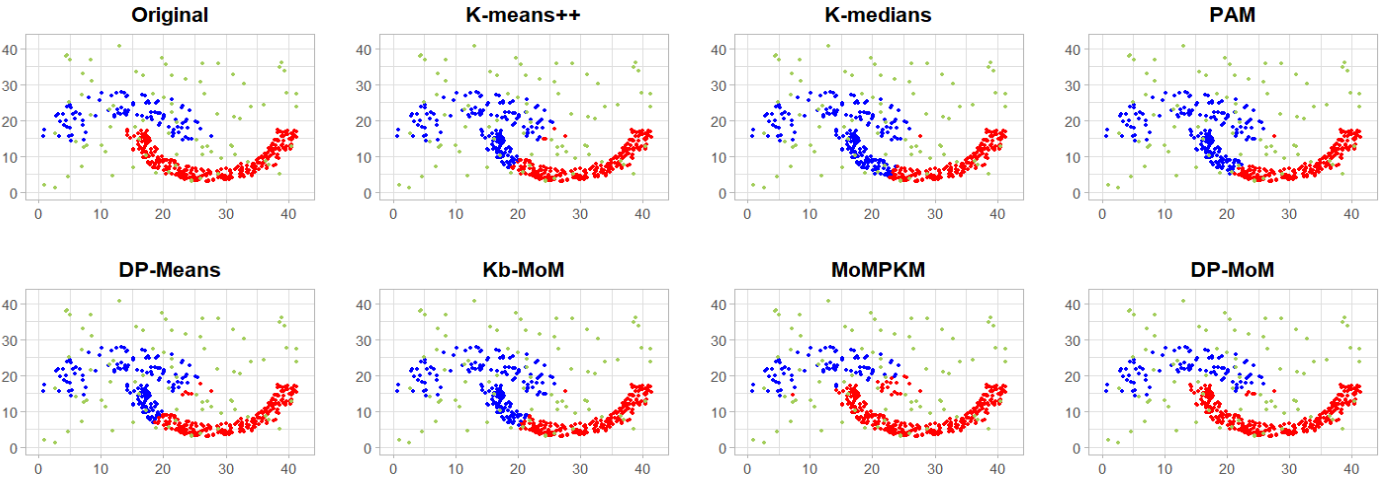
\includegraphics[width = \textwidth]{Diagrams/plot-jain-sim-comparison-0.7.png}
    \caption{Several state-of-the-art clustering methods fail to achieve proper clustering in presence of noisy observations (light green in color), while the performance of DP-MoM, our proposed algorithm, is nearly optimal.}
    \label{fig:jain-out}
\end{figure*}

In this article, we address these challenges by fusing two prominent clustering methodologies: centroid-based and model-based. Our proposed algorithm, DP-MoM, is meticulously designed to excel in scenarios involving noisy or outlier-affected data, courtesy of its utilization of the Median-of-Means (MoM) estimator \citep{nemirovsky1983wiley,devroye-MoM}. Additionally, DP-MoM offers the advantage of not necessitating a predefined number of clusters. To demonstrate the efficacy of our approach, we present a compelling example. We introduce randomly generated noisy observations into the \textit{Jain} dataset \citep{jain-dataset} (refer to the Experiments section for detailed information) and subsequently apply various cutting-edge algorithms, including our proposed DP-MoM, to evaluate their respective performances on the original dataset. As illustrated in Figure \ref{fig:jain-out}, DP-MoM showcases notably superior clustering accuracy compared to existing algorithms.



\section{Background}
\label{gen_inst}

\subsection{Clustering based on Dirichlet Process}

\cite{DP-Means} introduced a method utilizing Gibbs sampling, serving as a Bayesian counterpart to representing $k$-means with a mixture of Gaussians. We assume the following model to capture the cluster structure of the dataset and whose limiting case reduces to the Dirichlet Process Mixture models:
\begin{align*}
\boldsymbol{\theta}_1, \ldots, \boldsymbol{\theta}_{{k}} & \sim {G}_0, \\
\pi & \sim \operatorname{Dir}\left({k}, \pi_0\right), \\
{z}_1, \ldots, {z}_{{n}} & \sim \operatorname{Discrete}(\pi), \\
{\bX}_1, \ldots, {\bX}_{{n}} & \sim \mathcal{N}\left(\boldsymbol{\theta}_{{z}_{{i}}}, \sigma I\right),
\end{align*}
where $\boldsymbol{\theta}_{{j}}$ 's are the cluster centroids, ${G}_0$ is taken to be a $\mathcal{N}(0, \rho \mathbf{I})$ prior where $\mathbf{I}$ denotes the identity matrix of appropriate order. $\operatorname{Dir}\left({k}, \pi_0\right)$ denotes the Dirichlet distribution, where $\pi$ is the mixture probability with $\pi_0=\frac{\alpha}{k} \mathbf{1}$. Here, $\mathbf{1}$  denotes the vector (of appropriate order) of all $1$'s. For $i = 1,2,\ldots,n$, ${z}_{{i}}$ denotes the label assigned to the data points ${\bX}_{{i}}$, and  $\operatorname{Discrete}(\pi)$ indicates that ${z}_{{i}}$ takes the value $j$ with probability $\pi_{{j}}$, for ${j}=1, \ldots, {k}$.

The hard clustering algorithm, called \textit{DP-means}, proposed by \cite{DP-Means} is essentially the case when $\sigma \to 0$. This limiting case boils down to minimizing the objective:

\begin{equation}\label{dp-means-obj}
    f_{\operatorname{DP}} (\bTheta, k)=\sum_{i=1}^n \min _{1 \leq j \leq k}\left\|{\bX}_i-\boldsymbol{\theta}_j\right\|_2^2+\lambda k.
\end{equation}

The minimization of the function in \eqref{dp-means-obj} with respect to $k$ is performed iteratively. At each step of the algorithm, the distance from each data point to its closest cluster centroid is determined. Subsequently, each point is assigned to the cluster with the closest centroid, unless this distance exceeds $\lambda$. In such an instance, a new cluster is initialized with the data point serving as the centroid of the newly created cluster. This algorithm determines the number of clusters in a dataset without necessitating prior knowledge of $k$. It maintains the simplicity inherent in Lloyd's approach, while ensuring effectiveness even in situations where the true number of clusters is unknown.


\subsection{Median-of-Means (MoM)}

Let us consider a simple scenario first where we observe $\bX_1,\bX_2,\ldots,\bX_n\sim F$ with a goal to estimate the mean of the distribution $F$, i.e., $\mu_0=\mathbb{E} [\bX_1]=\int x\,dF(x)$.

We employ the median-of-means (MoM) estimator to estimate $\mu_0$ as follows: Assume that the sample size $n=bL$ where $L$ is the number of buckets (subsamples) and $b$ is the size of each bucket. We first split the data randomly into $L$ partitions (or buckets), and calculate the mean of the data points belonging to each partition. This gives rise to estimators $\hat{\mu}_1,\hat{\mu}_2,\ldots,\hat{\mu}_L$. The MoM estimator defined to be the median of these $b$ many mean estimators, namely,

\begin{equation}\label{MoM-defn}
\hat{\mu}_{\text{MoM}}=\operatorname{median} (\hat{\mu}_1,\hat{\mu}_2,\ldots,\hat{\mu}_L).
\end{equation}

In case of centroid-based clustering, the median-of-means estimator is used as follows: We first partition the dataset into $L$ subparts. In each iteration, we calculate the mean objective function value for each bucket $l$, $\frac{1}{b}\sum_{i \in B_{l}}f_{{\Theta}}(\bX_i)$ (where $\Theta$ is the collection of centroids from the previous iteration) and choose the bucket $L_t$ in such a way that
\begin{equation}\label{eq4}
    \frac{1}{b}\sum_{i \in B_{L_t}}f_{{\bTheta}}(\bX_i)=\operatorname{median}\left\{\displaystyle \frac{1}{b}\sum_{i \in B_{l}}f_{{\bTheta}}(\bX_i)\right\},\text{ }l=1,\ldots,L.
\end{equation}
The centroids $\Theta$ are recalculated based on the observations in the bucket $B_{L_t}$ and all the observations are clustered using these centroids.

A reason why this estimator is of such interest (apart from being a robust estimator) is that given $\operatorname{var}(\bX_1)=\sigma^2<\infty$ in the finite sample case, it satisfies the following concentration inequality \citep{lerasle2019lecture}: 
\begin{equation}
    P(|\hat{\mu}_\text{MoM}-\mu_0| > \epsilon) \leqslant e^{-2L} \left(\frac{1}{2}-\frac{L}{n}\frac{\sigma^2}{\epsilon^2}\right)^2 \text{for all } n=bL.
\end{equation}


\section{Dirichlet Process Clustering with MoM}

\subsection{Problem Formulation}
The problem posed to us is that of partitioning a given dataset $\mathcal{X} = \{\bX_1, \bX_2, \ldots, \bX_n\}\subset \mathbb{R}^p$ into natural, disjoint clusters such that the variance within each cluster is minimized at the same time maximizing the inter-partition variability. 


In the context of centroid-based clustering, the $j^{th}$ cluster is represented by its centroid $\boldsymbol{\theta}_j$. The concept of "closeness" is quantified by utilization of a Bregman divergence \citep{BREGMAN1967200} as a dissimilarity measure. Let us denote the set of all non-negative real numbers by $\mathbb{R}^{+}_0$. Any function $\phi: \mathbb{R}^p \rightarrow \mathbb{R}$ that is convex and differentiable, gives rise to the Bregman divergence $d_\phi: \mathbb{R}^p \times \mathbb{R}^p \rightarrow \mathbb{R}^{+}_0$ defined as
\begin{equation}
    d_\phi(\boldsymbol{x}, \boldsymbol{y})=\phi(\boldsymbol{x})-\phi(\boldsymbol{y})-\langle\nabla \phi(\boldsymbol{y}), \boldsymbol{x}-\boldsymbol{y}\rangle.
\end{equation}

The Bregman divergence that we shall be using in our framework is the Euclidean distance, generated by $\phi(\boldsymbol{u})=\|\boldsymbol{u}\|_2^2$. Prior knowledge of the number of centroids $k$ enables us to accomplish clustering by minimizing the objective
\begin{equation}\label{ob}
    f_{\boldsymbol{\Theta}}(\boldsymbol{X}) := \frac{1}{n} \sum_{i=1}^n \Psi\left(d_\phi\left(\boldsymbol{X}_i, \boldsymbol{\theta}_1\right), d_\phi\left(\boldsymbol{X}_i, \boldsymbol{\theta}_2\right), \ldots, d_\phi\left(\boldsymbol{X}_i, \boldsymbol{\theta}_k\right)\right).
\end{equation}

Here, $\Psi: {\mathbb{R}^{+}_0}^k \rightarrow \mathbb{R}^{+}_0$ is the function $\min_{1\le j\le k} d_{\phi}(\bm{X},\bm{\theta}_j)$. In our case, we will seek to minimize the objective function
\begin{equation}\label{obj}
    \operatorname{median}\left(\frac{1}{b} \sum_{i \in B_1} f_{\boldsymbol{\Theta}}\left(\boldsymbol{X}_i\right), \frac{1}{b} \sum_{i \in B_2} f_{\boldsymbol{\Theta}}\left(\boldsymbol{X}_i\right), \ldots, \frac{1}{b} \sum_{i \in B_L} f_{\boldsymbol{\Theta}}\left(\boldsymbol{X}_i\right)\right) + \lambda k
\end{equation}
with respect to both $\{\bm{\theta_j}\}_{1\le j\le k}$ and $k$.


\subsection{Optimization}

Optimizing the above objective is achieved using gradient-based methods. In our case, we employ the \textit{AdaGrad} algorithm \citep{duchi2011adaptive} for the said purpose. The centroids are updated as follows:
\begin{equation}
    \boldsymbol{\theta_j}^{(t+1)} := ~\boldsymbol{\theta}_j^{(t)} - \dfrac{\eta}{\sqrt{\varepsilon + \sum_{t' = 1}^t ||g_j^{(t')}||^2}} \cdot g_j^{(t)},
\end{equation}
where 
\begin{equation}
    g_j^{(t)} = \frac{1}{b}\sum_{i \in B_{l_t}} 2(\boldsymbol{\theta}_j^{(t)} - \bX_i)\cdot \mathbf{I}_{\{\bX_i \in \mathcal{C}_j\}}
\end{equation}
with 
\begin{equation}
    \mathbf{I}_{\{\bX_i \in \mathcal{C}_j\}}=\begin{cases}
1, & \text{if $u_{ij} = 1$}\\
0, & \text{otherwise.}
\end{cases}
\end{equation}

\subsection{Algorithm}

\begin{breakablealgorithm}%[!htb]
\caption{Dirichlet Process Means using Median-of-Means (DP-MoM)}
\label{algo1}
\flushleft{
\vspace{-2mm}\textbf{Data}: Data matrix $\mathcal{X}$, Penalty parameter $\lambda$, $\epsilon$, Learning Rate $\eta$, Tolerance $\delta$.\\
\textbf{Result}: Number of clusters $k$, Cluster assignments $\mathcal{U}$, Cluster centroids $\bTheta$.\\
\textbf{Initialization}: Randomly divide $\{1,\dots,n\}$ into $L$ buckets of equal size. 
Set $\boldsymbol{\theta_1}=\frac{1}{n}\sum_{i = 1}^{n} \bX_i$, $k=1$, $b=\frac{n}{L}$, and $\mathcal{U}=\mathbf{1}$.\\
}
\vspace{2mm}
\begin{algorithmic}[1]
% \SetAlgoLined
 \While{$t<t_{\text{max}}$ \text{or stopping condition is not satisfied}}
  % instructions\;
  \For{every observation $\bX_i$}
  \State Compute $a_i$= $\min\left\{\|\bX_i - \boldsymbol{\theta_j}\|^2,~j = 1,\cdots,k\right\}$
  \If{$a_i > \lambda$}
  \State Set $k=k+1$, $\btheta_k=\bX_i$
  \State Update $\mathcal{U}$ by $u_{ij} = \begin{cases} 1, \text{ if } j=k\\ 0, \text{ otherwise} \end{cases}$
% \ENDIF
   \Else
   \State Update $\mathcal{U}$ by $u_{ij}=\begin{cases} 1, \text{ if } j=\argmin_{1\leq c\leq k} ||\bX_i - \boldsymbol{\theta_c}||^2\\ 0, \text{ otherwise}\end{cases}$
   \EndIf
   \EndFor
  \State Find $l_t \in \{1, 2, ... , L\}$ such that $\displaystyle\frac{1}{b}\sum_{i \in B_{l_t}} f_{\boldsymbol{\Theta^{(t)}}}(\bX_i) = \displaystyle\operatorname{median}_{1\leqslant j\leqslant L} \left\{\displaystyle \frac{1}{b}\sum_{i \in B_{j}}f_{{\bTheta}}(\bX_i)\right\}$
  \State For each $j\in \{1, 2, ..., k\}$: $\displaystyle g_j^{(t)} = \displaystyle\frac{1}{b}\sum_{i \in B_{l_t}} 2(\boldsymbol{\theta}_j^{(t)} - \bX_i)u_{ij}$
  \State Update ${\Theta}$ by $\displaystyle\boldsymbol{\theta_j}^{(t+1)} := ~\boldsymbol{\theta}_j^{(t)} - \dfrac{\eta}{\sqrt{\varepsilon + \sum_{t' = 1}^t ||g_j^{(t')}||^2}} \cdot g_j^{(t)}$
 \EndWhile
\end{algorithmic}
\end{breakablealgorithm}




% $$\text{THE ALGORITHM WILL BE STATED HERE}$$

Algorithm \ref{algo1} summarizes the pseudocode for the above procedure. The tuning parameter $\epsilon$ is set to 1. The learning rate $\eta$ is typically chosen to be the power of 10 which is of the order of the square of the maximum pairwise distance in the dataset, or one lower than that i.e. if the maximum squared separation between any two observations in the data is $D$, then we set $\eta = 10 ^{\lceil 2\log_{10} D \rceil /2}$ or $10^{\lceil 2\log_{10} D \rceil /2-1}$ depending on which of these values aids efficient clustering using our proposed method, where $\lceil \cdot \rceil$ represents the ceiling function. Our proposed framework enables us to automatically detect the appropriate number of clusters based on the value of the penalty parameter $\lambda$ which is optimized by grid-searching.

\subsection{Parameter Selection}
The first step in our proposed algorithm is partitioning the dataset randomly. This is achieved by choosing a permutation of the data points uniformly and then placing them in different buckets in the order of the permutation. Though this technique achieves randomness in terms of partitioning the data, arbitrary partitioning may lead to undesirable results, which is why the partitioning (or permutation for that matter) needs to be carefully chosen. We resort to a form of grid search to solve this problem. We determine $\lambda_{\min}$ and $\lambda_{\max}$, the minimum and maximum pairwise squared distance between the data points, respectively. $11$ equally-spaced points $\lambda_{\min} =\lambda^1_1<\lambda^1_2< \cdots < \lambda^1_{10}<\lambda^1_{11}=\lambda_{\max}$ are picked, and the algorithm is run for these values and for all values of number of partitions, $L$, such that $2<L<\frac{n}{3}$. We select $\lambda^1_{i^*}$ corresponding to the most accurate clustering and divide its neighborhood $[\lambda^1_{i^*-1},\lambda_{i^*-1}]$  $\left([\lambda^1_1,\lambda^1_2]\operatorname{ or }[\lambda^1_{10}, \lambda^1_{11}]\right)$ into $20$ divisions and re-run the algorithm as we did in the interval $[\lambda_{\min}, \lambda_{\max}]$. We repeat this one more time, so that the feasible range for the penalty parameter $\lambda$ has been segmented to the order of $10^3$. We obtain the permutation corresponding to the most accurate clustering in the three stages above, and use this particular permutation to partition the data for further experiments.

We imitate the above experiment, except that this time we use the permutation of the data points that have been obtained from the said grid-searching, to partition the data. We then choose the $\lambda$ and $L$ values for which the best clustering accuracy is attained. We call them $\lambda_{opt}$ and $L_{opt}$. Since our proposed algorithm is a randomized one, we cannot readily conclude that $\lambda_{opt}$ and $L_{opt}$ are the only values corresponding to which we will obtain high clustering accuracy. In fact, for another repetition of the above experiment, we may not obtain an identical favorable permutation or the same optimal $\lambda$ and $L$ values. So, we repeat the aforementioned grid-searching experiment a number of times (say about 30 times) so that we may obtain a range of $\lambda$ and a range of $L$ that will be suitable to work with in order to derive the best results out of the proposed framework. We choose the median of the clustering accuracies, measured with the Adjusted Rand Index (ARI) \citep{Hubert1985} so obtained, as a representative of the clustering accuracy of the algorithm.

\subsection{Computational Complexity}
% \textcolor{red}{$\mathcal{O}(nKp)$ per iteration}
In each iteration, our algorithm first ascertains whether an increase in the number of clusters is needed. The centroids are recalculated thereafter, and the cluster assignments are made accordingly. This phase typically takes $\mathcal{O}(nCp)$ time steps to complete, where $C$ represents the number of clusters in that iteration. The calculations presented in the following section assume that the number of clusters is upper bounded by some finite $K<n$. Consequently, the worst case runtime of the DP-MoM algorithm remains $\mathcal{O}(nKp)$ for every iteration.

The computational complexity of the DP-means algorithm is comparable to that of DP-MoM, as each iteration requires $\mathcal{O}(nCp)$ steps to complete, with $C$ denoting the number of clusters in that specific iteration. On the contrary, $k$-means demands $\mathcal{O}(nkp)$ steps per iteration, with $k$ representing the predefined cluster count. This is typically slated to be lower than that of DP-means or DP-MoM. In the case where we set $k=K$ however, $k$-means will perform no more efficiently than DP-MoM in terms of runtime.


\section{Theoretical Results}
\label{sec:theory}

% We seek to minimize the objective function (\ref{obj}) with the assumption that we will stop updating the clusters when the total number of clusters reach a maximum value of $K$. Then we can derive the finite sample error bounds for the method, similar to \cite{paul2021uniform}. 

% \begin{assumption}\label{a1}
% $\bX_1\dots,\bX_n \overset{i.i.d.}{\sim} P$ such that $P \in \mathcal{M}$.
% \end{assumption}

% \begin{assumption}\label{a2}
%     The number of clusters $k$ is bounded above by some positive constant $K$, where $K<n$.
% \end{assumption}

% Let $P_n$ denote the empirical distribution derived from the data $\bX_1\ldots,\bX_n$. In other words, for any Borel set $A$, $P_n(A) = \frac{1}{n}\sum_{i=1}^n \mathbf{I}\{\bX_i \in A\}$. 
% To simplify notation, we use $\mu f := \int f d\mu$. 

% By utilizing the Strong Law of Large Numbers (SLLN) as presented in \cite{athreya2006measure}, we can conclude that $P_n f_{\bTheta}$ converges almost surely to $Pf_{\bTheta}$, where the objective \ref{obj} can be reformulated as a constrained minimization, 


% \begin{equation}
%     \operatorname{median}\left(\frac{1}{b} \sum_{i \in B_1} f_{\boldsymbol{\Theta}}\left(\boldsymbol{X}_i\right), \ldots, \frac{1}{b} \sum_{i \in B_L} f_{\boldsymbol{\Theta}}\left(\boldsymbol{X}_i\right)\right),\quad\text{subject to, } k\leq K.
% \end{equation}


Let us denote the set of all probability measures $P$ with support on $[-M,M]^p$ by $\mathcal{M}$%, i.e., $P\left([-M,M]^p\right)=1$ $\forall$ $P\in \mathcal{M}$
. We shall make a standard assumption that all the data points are independent and identically distributed (\textit{i.i.d.}) with bounded components.

\begin{assumption}\label{ass-1-iid}
    $\bm{X}_1,\bm{X}_2,\ldots,\bm{X}_n \overset{\text{iid}}{\sim}P$ such that $P\in \mathcal{M}$.
\end{assumption}

We denote the empirical distribution derived from $\bX_1\ldots,\bX_n$, by $P_n$, that is, $P_n(A) = \frac{1}{n}\sum_{i=1}^n \mathbf{I}\{\bX_i \in A\}$ for any Borel set $A$. 
For the sake of notational simplicity, we write $\mu f := \int f \, d\mu$. Thanks to the Strong Law of Large Numbers (SLLN) presented in \cite{athreya2006measure}, we can conclude that $P_n f_{\bTheta} \rightarrow Pf_{\bTheta}$ almost surely. Let $\widehat{\bm{\Theta}}_n$ be a minimizer of \[f_{\bm\Theta}(\bm{X})=\frac{1}{n} \sum_{i=1}^n \Psi(d_{\phi}(\bm{X}_i, \bm{\theta}_1), d_{\phi}(\bm{X}_i, \bm{\theta}_2), \ldots, d_{\phi}(\bm{X}_i, \bm{\theta}_k)),\]
and $\bm{\Theta}^*$ be the global minimizer of $Pf_{\bm{\Theta}}$. 
Owing to the fact that $P_n f_{\bm{\Theta}}$ and $P f_{\bTheta}$ are close for large enough $n$, it is reasonable to expect that the absolute difference between $\widehat{\bm{\Theta}}_n$ and $\bm{\widehat{\Theta}}^*$ will be small. %To show that $\bm{\widehat{\Theta}}_n$ converges to $\bm{\Theta}^*$ as $n\to \infty $, we consider bounding the uniform deviation $\sup_{\bm{\Theta}}|P_n f_{\bm{\Theta }}-Pf_{\bm{\Theta}}|$.

\begin{assumption}\label{ass-2-cluster-count}
    The number of clusters $k$ is bounded above by some finite $K\in \mathbb{N}$, where $K < n$.
\end{assumption}

The inherent dependency of the number of centroids on the cluster penalty parameter $\bm{\lambda}$ makes it possible for us to choose $\bm{\lambda}$ appropriately so that the cluster count doesn't exceed $K$. Moreover, we deduce from A\ref{ass-2-cluster-count} that, at a certain juncture, the number of centroids reaches a state of stability. In this state, it is only the cluster centroids themselves that undergo updates during each iteration, while the number of centroids remains constant. This will make our analysis independent of the penalty parameter $\bm{\lambda}$ as the term $k\bm{\lambda}$ is not subject to change after a finite number of iterations. Consequently, beyond a finite number of steps, the objective function effectively reduces to 
\begin{equation}\label{DP-MoM-obj}
    \operatorname{MoM}_L^n(\bTheta) := \operatorname{median} \left(\frac{1}{b}\sum_{i\in B_{1}}f_{\bm{\Theta}}(\bm{X}_i), \frac{1}{b}\sum_{i\in B_{2}}f_{\bm{\Theta}}(\bm{X}_i), \ldots, \frac{1}{b}\sum_{i\in B_{\ell}}f_{\bm{\Theta}}(\bm{X}_i)\right).
\end{equation} 

\begin{remark}
    In our framework, $\displaystyle |\Psi(\bm{x})-\Psi(\bm{y})|\le \|\bm{x}-\bm{y}\|_1$.
\end{remark}

To see this, recall the definition of $\Psi$ in \eqref{obj}, and note that $|\Psi(\bm{x})-\Psi(\bm{y})|=|\min_{1\le j\le K}x_j-\min_{1\le j\le K}y_j|$. Let us assume, without loss of generality, that $\min_{1\le j\le K}x_j\ge \min_{1\le j\le K}y_j$. Hence, $\min_{1\le j\le K}x_j-\min_{1\le j\le K}y_j\le x_{j^*}-y_{j^*}\le \|\bm{x}-\bm{y}\|_1$ where $j^* = \operatorname{argmin}_{1\le j\le K}y_j$ and the remark is seen to hold.

% \begin{lemma}\label{lemma-a1-lipschitz}
%     For $\bm{x},\bm{y}\in [-M,M]^p$, $\phi(\bm{u})=\|\bm{u}\|_2^2$ is $2M\sqrt{p}$-Lipschitz i.e. \[|\phi(\bm{x})-\phi(\bm{y})|\le 2M\sqrt{p}\|\bm{x}-\bm{y}\|_2\]
% \end{lemma}


% Then it is equivalent to solving the unconstrained minimization problem with $K$ many clusters. Hence,
% \begin{equation}
%     P_nf_{\bTheta}=\operatorname{median}\left(\frac{1}{b} \sum_{i \in B_1} f_{\boldsymbol{\Theta}}\left(\boldsymbol{X}_i\right), \ldots, \frac{1}{b} \sum_{i \in B_L} f_{\boldsymbol{\Theta}}\left(\boldsymbol{X}_i\right)\right)
% \end{equation}

% Thus, the optimization problem becomes equivalent to MoMPKM \cite{paul2021uniform}. Thus, under the same assumptions $A1-A6$ of \cite{paul2021uniform}, for a fixed number of features $p$, with probability at least $1-\delta$ for some $\delta>0$, the following holds.
% \begin{equation}
%     |Pf_{\hat{\bTheta}_n} - P f_{\bTheta^\ast}|  \le 192 \sqrt{\pi} \tau_{\balpha, K} H_p M^2  (Kp)^{3/2} n^{-1/2} + 8 \tau_{\balpha, K} H_p M^2 p K \sqrt{\frac{\log(2/\delta)}{2n}}.
% \end{equation}
% Here, $\hat{\bTheta}_n$ is the empirical minimizer, $\bTheta^\ast$ is the global population minimizer, $\tau_{\balpha, K}$ is a Lipschitz constant for the function $\Psi_\alpha$ defined in (\ref{psi}), $M$ is a positive constant which comes from the assumption that $\bTheta^\ast \in \mathscr{G}$. 

% \begin{remark}
% For constant $p$ and $K$, the finite sample error rate becomes $O_P (n^{-1/2})$. Also, in this case, $\hat{\bTheta}_n \xrightarrow{a.s.} \bTheta^\ast$. 
% \end{remark}
% \begin{remark}
%     If $K$ varies and is of the order $\log n$, then the error rate becomes $\mathcal{O}_P\left(\sqrt{(\log n)^3/n}\right)$.
% \end{remark}
% If $K$ varies, for fixed $p$, the error bound is $\mathcal{O}_P\left(\sqrt{K^3/n}\right)$. Thus, for the error to asymptotically go to zero, we must have $K$ such that $\lim_{n\rightarrow \infty} \frac{K^3}{n} = 0$. In general, for varying $p$, the finite sample error bound is $\mathcal{O}_P((Kp)^{3/2}n^{-1/2})$, hence we must have $\lim_{n\rightarrow \infty} \frac{(Kp)^3}{n} = 0$.

% \begin{lemma}\label{lemma-a2}
%     Under A\ref{ass-1-iid} and A\ref{ass-2-cluster-count}, for any $\bm{\Theta}, \bm{\Theta'}\in [-M,M]^p$, \[\|f_{\bm{\Theta}} - f_{\bm{\Theta'}}\|_{\infty}\le 4M\sqrt{p}\sum_{j=1}^{K}\|\bm{\theta}_j-\bm{\theta}_j'\|_2\]
% \end{lemma}


% \subsection{Bounding the minimizers \texorpdfstring{$\widehat{\bm{\Theta}}_n$}{theta-hat-n} and \texorpdfstring{$\bm{\Theta}^*$}{theta-star}}

\subsection{Concentration Inequalities on the Empirical Measure through Rademacher Complexity}

We start off by defining $\mathscr{G} := [-M,M]^{K \times p}$. To show that $\displaystyle \widehat{\bm{\Theta}}_n$ converges to $\bm{\Theta}^*$ as $n \to \infty$, the first step is to prove that both $\widehat{\bm{\Theta}}_n$ and $\displaystyle \bm{\Theta}^*$ lie in $\mathscr{G}$. We begin by stating the following result.

% \begin{lemma}\label{lemma-1-obtuse}
%     Let $\mathcal{C}$ be a convex set, and suppose $P_{\mathcal{C}}(\bm{\theta})$ be the projection of $\bm{\theta}$ onto $\mathcal{C}$, with respect to the Bregman divergence $d_{\phi}(\cdot,\cdot)$ i.e. $P_{\mathcal{C}}(\bm{\theta})=\operatorname{argmin}_{\bm{x}\in \mathcal{C}}d_{\phi}(x,\bm{\theta})$ (assuming it exists). Then \[d_{\phi}(\bm{x}, \bm{\theta})\ge d_{\phi}(\bm{x}, P_{\mathcal{C}(\bm{\theta})})+d_{\phi}(P_{\mathcal{C}(\bm{\theta})}, \bm{\theta})\hspace{0.3cm}\text{ for all }\bm{x}\in \mathcal{C}.\]
% \end{lemma}

\begin{lemma}\label{lemma-1-obtuse}
    Consider a convex set $\mathcal{C}$ and let $P_{\mathcal{C}}(\bm{\theta})$ be the projection of $\bm{\theta}$ onto $\mathcal{C}$ with respect to $d_{\phi}(\bm{x},\bm{\theta})=\|\bm{x}-\bm{\theta}\|_2^2$, i.e., $P_\mathcal{C}(\bm{\theta})=\operatorname{argmin}_{\bm{x}\in \mathcal{C}}\|\bm{x}-\bm{\theta}\|_2^2$. Then \[\|\bm{x}-\bm{\theta}\|_2^2\ge \|\bm{x}-P_{\mathcal{C}}(\bm{\theta})\|_2^2+\|P_{\mathcal{C}}(\bm{\theta})-\bm{\theta}\|_2^2.\]
\end{lemma}

Lemma \ref{lemma-1-obtuse} follows directly from the obtuse angle property presented in Section 3 of \cite{paul2021a}, by setting $d_\phi$ to be the squared Euclidean distance. We next show that for minimizing $P_n f_{\bm{\Theta}}$ or $P f_{\bm{\Theta}}$, it is enough to restrict our search space to $\mathscr{G}$.

\begin{lemma}\label{lemma-2}
    Let $Q \in \mathcal{M}$. For any $\bm{\Theta} \in \mathbb{R}^{K \times p}$, there exists $\bm{\Theta}^{\prime} \in\mathscr{G}$, such that $Q f_{\bm{\Theta^{\prime}}} \leq Q f_{\bm{\Theta}}$.
\end{lemma}

Since we can restrict our attention to $\mathscr{G}$ to minimize $Q f_{\bm\Theta}$, we have the following:

\begin{cor}
    Let $Q \in \mathcal{M}$. If $\bm{\Theta}_0=\argmin_{\bm{\Theta} \in \mathbb{R}^{K \times p}} \int f_{\bm{\Theta}} \,dQ$, then $\bm{\Theta}_0 \in \mathscr{G}$.
\end{cor}

Note that under A\ref{ass-1-iid} and A\ref{ass-2-cluster-count}, both $P$ and $P_n$ have support contained in $\mathscr{G}$. Corollary \ref{cor-4.2} follows from the preceding by replacing $Q$ by $P$ and $P_n$.

\begin{cor}\label{cor-4.2}
    Under A\ref{ass-1-iid}--A\ref{ass-2-cluster-count}, both $\widehat{\boldsymbol{\Theta}}_n, \boldsymbol{\Theta}^* \in \mathscr{G}$.
\end{cor}

%Now that we have bounded $\widehat{\bm{\Theta}}_n$ and $\bm{\Theta}^*$ in a compact set, the following section supplies probabilistic bounds on the uniform deviation $2 \sup _{\bm{\Theta} \in\mathscr{G}}\left|P_nf_{\bm\Theta} - Pf_{\bm{\Theta}}\right|$ via metric entropy arguments.


% \subsection{Concentration Inequality and Metric Entropy Bounds via Rademacher Complexity}

%We have proven that $\widehat{\boldsymbol{\Theta}}_n, \boldsymbol{\Theta}^* \in\mathscr{G}$. 
Next, we observe that
% \begin{align*}
%     |P f_{\widehat{\bm{\Theta}}_n}- P f_{\bm{\Theta^*}}|
%     = P f_{\widehat{\bm{\Theta}}_n}- P f_{\bm{\Theta^*}} 
%     &= P f_{\widehat{\bm{\Theta}}_n}-P_n f_{\widehat{\bm{\Theta}}_n}+P_n f_{\widehat{\bm{\Theta}}_n}-P_n f_{\bm{\Theta^*}}+P_n f_{\bm{\Theta^*}} - P f_{\bm{\Theta^*}}\\
%     &\le P f_{\widehat{\bm{\Theta}}_n}-P_n f_{\widehat{\bm{\Theta}}_n}+P_n f_{\bm{\Theta^*}} - P f_{\bm{\Theta^*}}\\
%     &\le 2\sup_{\bm{\Theta}\in \mathscr{G}}|P_n f_{\bm\Theta}-P f_{\bm\Theta}|
% \end{align*}
\begin{equation}
    |P f_{\widehat{\bm{\Theta}}_n}- P f_{\bm{\Theta^*}}|
    = P f_{\widehat{\bm{\Theta}}_n}- P f_{\bm{\Theta^*}} 
    % = P f_{\widehat{\bm{\Theta}}_n}-P_n f_{\widehat{\bm{\Theta}}_n}+P_n f_{\widehat{\bm{\Theta}}_n}-P_n f_{\bm{\Theta^*}}+P_n f_{\bm{\Theta^*}} - P f_{\bm{\Theta^*}}\\
    \le P f_{\widehat{\bm{\Theta}}_n}-P_n f_{\widehat{\bm{\Theta}}_n}+P_n f_{\bm{\Theta^*}} - P f_{\bm{\Theta^*}}\\
    \le 2\sup_{\bm{\Theta}\in \mathscr{G}}|P_n f_{\bm\Theta}-P f_{\bm\Theta}|.
\end{equation}

Towards bounding $|P f_{\widehat{\bm{\Theta}}_n}-P f_{\bm{\Theta}^*}|$, it suffices to bound the quantity $\sup _{\bm{\Theta} \in\mathscr{G}}\left|P_n f_{\bm\Theta} - P f_{\bm\Theta}\right|$. Employing the Rademacher complexity \citep{DUDLEY1967290,FoML-mohri}, we constrain this deviation and subsequently establish an upper bound on the Rademacher complexity. Let $\mathcal{F}=\left\{f_{\bm\Theta}: \bm{\Theta} \in\mathscr{G}\right\}$. Also, define the $\mathcal{F}$-norm $\|\mu-\nu\|_{\mathcal{F}}$ between two probability measures $\mu$ and $\nu$ \citep{athreya2006measure} by $ \sup_{f \in \mathcal{F}}\left|\int f \,d\mu-\int f \,d\nu\right|$. Recall that the Rademacher complexity is defined as follows:

\begin{defn}
    (Rademacher complexity) Let $\epsilon_i$'s be i.i.d. Rademacher random variables independent of $\mathcal{X}=\left\{\boldsymbol{X}_1, \ldots, \boldsymbol{X}_n\right\}$, i.e. $\mathbb{P}\left(\epsilon_i=1\right)=\mathbb{P}\left(\epsilon_i=-1\right)=0.5$, The population Rademacher complexity of $\mathcal{F}$ is defined as $\mathcal{R}_n(\mathcal{F})=\E\sup _{f \in \mathcal{F}} \frac{1}{n} \sum_{i=1}^n \epsilon_i f\left(\boldsymbol{X}_i\right)$, where the expectation is over both $\epsilon$ and $\mathcal{X}$.
\end{defn}

\begin{comment}
\begin{defn}
    ($\delta$-cover and Covering Number) Let $(X, d)$ be a metric space. The set $X_\delta \subseteq X$ is said to be a $\delta$-cover of $X$ if for all $x \in X, \exists$ $x^{\prime} \in X_\delta$, such that $d\left(x, x^{\prime}\right) \leq \delta$. The $\delta$-covering number of $X$ w.r.t. $d$, denoted by $N(\delta ; X, d)$, is the size of the smallest $\delta$-cover of $X$ with respect to $d$.
\end{defn}

The following lemma gives a bound for the $\delta$-covering number of $\mathcal{F}$ under the supremum norm. The main idea here is to use the Lipschitz property of $f_{\Theta}$ and then to find a cover of the search space for $\Theta$, i.e. $\mathscr{G}$. This then automatically transcends to a cover of $\mathcal{F}$ under the sup-norm.

\begin{lemma}\label{lemma-3-cov-num}
    Let $N\left(\delta ; \mathcal{F},\|\cdot\|_{\infty}\right)$ be the $\delta$-covering number of $\mathcal{F}$ under $\|\cdot\|_{\infty}$. Then, under  assumptions A\ref{ass-1-iid} and A\ref{ass-2-cluster-count}, $$N\left(\delta ; \mathcal{F},\|\cdot\|_{\infty}\right) \leq\left(\max \left\{\left\lfloor\frac{4 M^2 K p}{\delta}\right\rfloor, 1\right\}\right)^{Kp}.$$
\end{lemma}

\begin{lemma}\label{lemma-4-diam}
    Let diam($\mathcal{F}$)=$\sup_{f,g\in \mathcal{F}}\|f-g\|_{\infty}$. Then under A\ref{ass-1-iid} and A\ref{ass-2-cluster-count}, diam($\mathcal{F}$) $\le 8M^2Kp$.
\end{lemma}
\end{comment}

% Lemma \ref{lemma-4-diam} puts an upper bound on the diameter of $\mathcal{F}$, defined above, under $\|\cdot\|_{\infty}$. 
Following \cite{paul2021uniform}, we can devise a bound on the Rademacher complexity $\mathcal{R}_n(\mathcal{F})$ as stated in Theorem \ref{thm-1-RnF}.

\begin{thm}\label{thm-1-RnF}
    Under A\ref{ass-1-iid}--A\ref{ass-2-cluster-count}, $\mathcal{R}_n(\mathcal{F})\le 48\sqrt{\pi}M^2(Kp)^{3/2}n^{-1/2}$.
\end{thm}

% Before we proceed further, we would like to state the following lemma which puts a uniform bound on $\|f\|_{\infty}$ for $f\in \mathcal{F}$.
\begin{comment}
\begin{lemma}\label{lemma-5}
    For all $x\in [-M,M]^p$ and $\bm{\Theta}\in \mathscr{G}$, \[0\le \Psi(d_{\phi}(\bm{x},\bm{\theta}_1), d_{\phi}(\bm{x},\bm{\theta}_2),\cdots, d_{\phi}(\bm{x},\bm{\theta}_K) )\le 4M^2p.\]
\end{lemma}
\end{comment}

Given the result stated in Theorem \ref{thm-1-RnF}, we seek a non-asymptotic bound on $|P f_{\widehat{\bm{\Theta}}_n}-Pf_{\bm{\Theta}^*}|$ by deriving a uniform concentration inequality on $\|P_n-P\|_{\mathcal{F}}$.

\begin{thm}\label{thm-2-diff-Pn-P}
    Under A\ref{ass-1-iid}--A\ref{ass-2-cluster-count}, for any $\delta\in(0,1)$, the inequality 
    \[\|P_n-P\|_\mathcal{F}\le \left[96\sqrt{\pi}M^2(Kp)^{3/2} + 4\sqrt{2} M^2p\log^{\frac{1}{2}}\big(\tfrac{2}{\delta}\big) \right] n^{-1/2}\]
    holds with probability at least $1-\delta$.
\end{thm}

% The result in Theorem \ref{thm-2-diff-Pn-P} reveals a non-asymptotic bound on $|P f_{\widehat{\bm{\Theta}}_n}-Pf_{\bm{\Theta}^*}|$:

\begin{cor}
    Under A\ref{ass-1-iid}--A\ref{ass-2-cluster-count}, for any $\delta\in(0,1)$, the inequality% the following holds: 
    \[|P f_{\widehat{\bm{\Theta}}_n}-Pf_{\bm{\Theta}^*}|\le \left[192\sqrt{\pi}M^2(Kp)^{3/2} + 8\sqrt{2} M^2p\log^{\frac{1}{2}}\big(\tfrac{2}{\delta}\big) \right] n^{-1/2}\]
    holds with probability at least $1-\delta$.
\end{cor}


\subsection{Asymptotic Properties: Strong Consistency and Rate of Convergence}

We now consider the classical setting where $p$ is held constant, and demonstrate that the previously presented results imply strong consistency, with rate of convergence of the order of $\mathcal{O}(n^{-1/2})$. We first follow the same idea of convergence of $\hth$ to $\bTheta^\ast$ that is outlined in \cite{pollard1981strong}. Since the centroids are unique up to rearrangement of labels, our concept of dissimilarity
\[\mathcal{D}(\bTheta_1,\bTheta_2) = \min_{M \in \mathscr{P}_K} \|\bTheta_1 - M \bTheta_2\|_F \]
is considered over $\mathscr{P}_K$ the set of all real permutation matrices of order $K$, where $\|\cdot\|_F$ represents the
Frobenius norm. The sequence $\bTheta_n\to \bTheta$ if $\lim_{n\to \infty} \mathcal{D}(\bTheta_n,\bTheta)=0$. Following \cite{terada2014strong,chakraborty2020entropy}, we assume the identifiablity condition:

\begin{assumption}\label{ass-3-diss}
    $\forall$ $ \eta>0$, $\exists$ $\epsilon>0$, such that $\, \mathcal{D}(\bTheta,\bTheta^\ast)> \eta$ $\implies$ $P f_{\bTheta} > P f_{\bTheta^\ast} + \epsilon$ .
\end{assumption}

We now examine the strong consistency of $\hth$. In addition, we analyze the rate at which $|P f_{\hth} - P f_{\bTheta^\ast}|$ approaches $0$. Theorem \ref{thm-3-strong-consistency} affirms that strong consistency holds, with $\mathcal{O}(n^{-1/2})$ rate of convergence. Before delving further, we must recall that $X_n = \mathcal{O}_P(a_n)$ if the sequence $X_n/a_n$ is bounded in probability.

\begin{thm}\label{thm-3-strong-consistency}
(Theorem 3.3 of \cite{paul2021uniform}) If $p$ is assumed to be constant then under  A\ref{ass-1-iid}--A\ref{ass-3-diss}, $\hth \xrightarrow{a.s.} \bTheta^\ast$ under $P$. Additionally, $|P f_{\hth} - P f_{\bTheta^\ast}| = \mathcal{O}_P (n^{-1/2})$.
\end{thm}


\subsection{Analysis under the Median-of-Means (MoM) Paradigm}

The results and analysis we have presented so far pertains to the situation where outlying or contaminating observations are absent. In this section, we assess the behavior of the centroids and the performance of Algorithm \ref{algo1} in the presence of outlying observations. %Without loss of generality, we assume $n=L\cdot B$. 
  We represent the set of all inliers as $\{\bX_i\}_{i \in \I}$ and the outliers as $\{\bX_i\}_{i \in \cO}$. Denoting the  minimizer of \eqref{eq4} by $\tm$, we make the following assumptions for determining the rate at which $|Pf_{\tm} - Pf_{\bTheta^\ast}|$ approaches $0$. % as a function of $n,\,p,\,k,\,L$ and $|\I|$. To this end, 

\begin{assumption}\label{ass-4-iid}
    $\{\bX_i\}_{i \in \I}\sim P$ are i.i.d. with $P \in \mathcal{M}$.
\end{assumption}

\begin{assumption}\label{ass-5-L}
    $\exists$ $\, \eta > 0$ such that $L>(2+\eta)|\cO|$.
\end{assumption}

It is important to note that A\ref{ass-4-iid} is exactly the same as A\ref{ass-1-iid}, but specifically applied to the inliers. A\ref{ass-5-L} guarantees that at least half of the $L$ partitions are devoid of outliers; which is a milder requirement compared to the condition $L > 4|\cO|$ imposed in the recent work \citep{lecue2020robust}. Crucially, we highlight that no distributional assumptions are imposed on the outliers, permitting them to be unbounded, originate from heavy-tailed distributions, or exhibit any sort of dependence structure among each other. We cite Lemma 4.6 and subsequent Corollary 4.4 from \cite{paul2021uniform}.

\begin{lemma}\label{lemma-6-spmom}
Under A\ref{ass-4-iid}-A\ref{ass-5-L}, for any $\bTheta \in \Real^{K\times p}$, $\exists$ $\bTheta^\prime \in \mathscr{G}$, such that $\text{MoM}_L^n(\bTheta^\prime) \le \text{MoM}_L^n(\bTheta)$.
\end{lemma}

\begin{cor}
Under A\ref{ass-4-iid}-A\ref{ass-5-L}, $\tm \in \mathscr{G}$.
\end{cor}

The above results confirm that the search space for $\tm$ may be constrained to $\mathscr{G}$. Subsequently, we establish a bound on $\sup_{\bTheta \in \mathscr{G}} |\text{MoM}^n_L (f_{\bTheta}) - Pf_{\bTheta} |$, and further use it to bound $|P f_{\tm} - P f_{\bTheta^\ast}|$. 
We %define $\delta:=2/(4+\eta) - |\cO|/L$, and 
use ``$\lesssim$'' to denote the fact that a quantity is lesser than a constant multiple of the other. % $\delta:= \frac{2}{4+\eta} - \frac{|\cO|}{L}$; 


\begin{thm}\label{thm-4-MoM}
Under A\ref{ass-4-iid}-A\ref{ass-5-L}, with probability at least $1-4e^{-L \delta^2/2}$, 
\[ \sup_{\bTheta \in \mathscr{G}} \left|\text{MoM}^n_L (f_{\bTheta}) - Pf_{\bTheta} \right| \lesssim  \max\left\{ Kp
L^{1/2}n^{-1/2}, (Kp)^{3/2}  |\I|^{1/2}n^{-1}\right\}.\]
\end{thm}

We present below a corollary that aids us in controlling the absolute difference $|P f_{\tm} - P f_{\bTheta^\ast}|$.

\begin{cor}
Under A\ref{ass-4-iid}-A\ref{ass-5-L}, with  probability at least $1-4e^{-L \delta^2/2}$,
\[ \left|P f_{\tm} - P f_{\bTheta^\ast}\right| \lesssim \max\left\{ KpL^{1/2}n^{-1/2}, (Kp)^{3/2} |\I|^{1/2}n^{-1}\right\}.\]
\end{cor}


\section{Experiments}
\label{sec:experiments}
We now empirically compare our proposed framework with existing clustering approaches to thoroughly validate and evaluate its effectiveness. The accuracy of cluster assignments has been rigorously assessed using the Adjusted Rand Index (ARI), a robust measure of clustering performance.
Our evaluation encompasses an extensive array of competing centroid-based clustering methods, including renowned techniques such as $k$-means$++$, Sparse $k$-means (SKM) \citep{SKM-paper}, $k$-medians, Partition around Medoids (PAM) \citep{PAM-paper}, Robust Continuous Clustering (RCC) \citep{Shah2017-jj}, DP-means \citep{DP-Means}, $k$-bootstrap Median-of-Means ($k$b-MoM) \citep{brunetsaumard2020kbmom}, Median-of-Means with Power $k$-means (MoMPKM), and Ordered Weighted $l_1$ $k$-means (OWL $k$-means) \citep{pmlr-v206-chakraborty23a}. These state-of-the-art algorithms are benchmarked against the proposed DP-MoM algorithm across various experimental scenarios. The simulation experiments were conducted using computer equipped with Intel(R) Core(TM)i3-7020U  2.30GHz  processor, 4GB RAM, 64-bit Windows 10 operating  system in the \texttt{R} programming language \citep{R-lang}.

Our first experiment involves implementing the aforementioned techniques on several datasets from the UCI Machine Learning Repository\footnote{\url{https://archive.ics.uci.edu/}} and the Compcancer database\footnote{\url{https://schlieplab.org/Static/Supplements/CompCancer/}}. Owing to the fact that our clustering technique relies on randomization while partitioning the data into buckets, the accuracy measure has been computed as the median value of the obtained ARI over $30$ test runs. It was observed, for most of the datasets, that DP-MoM performed considerably better than its competitors in terms of ARI. Apart from this, two other experiments were conducted to assess the strength of the algorithm in terms of robustness and ability to detect clusters of various shapes that were in proximity to one another in terms of their pairwise Euclidean distances.


\subsection{Simulation Studies}
% \paragraph{Introducing Outliers in Real Data} \newline

\paragraph{Study of Robustness on Simulated Data:} $30$ data points are generated from each of the $4$ quadrants in the $2$-dimensional Euclidean plane using a special generation scheme. For the first quadrant, we generate $R_i \sim U(0, 1)$ and $\theta_i \sim U\left(\frac{\pi}{36}, \frac{17\pi}{36}\right)$. Once this is done for all $i=1,2,\ldots,30$, we set $X_i = (R_i\cos\theta_i, R_i\sin \theta_i)$ for all $i=1,2,\ldots,30$ as our data points in the first quadrant. In the other quadrants, we draw $R_i$ in the same way and generate $\theta_i$ uniformly from $\left(\frac{(j - 1)\pi}{2} + \frac{\pi}{36}, \frac{j\pi}{2} - \frac{\pi}{36}\right)$ for the $j^{th}$ quadrant. We place the data points lying in the same quadrant in the same cluster. Just like in the experiment using the \textit{Jain} dataset, outliers have been generated uniformly on $[-1, 1] \times [-1, 1]$. $15, 15,$ and $20$ outliers were introduced in three stages, respectively, so that the total number of data points stood at $135$, $150$, and $170$ respectively. While the efficiency of the other competing algorithms plummeted or showed erratic behavior (often combined with low clustering accuracy), the ARI corresponding to DP-MoM did not waver. Figure 2 depicts the superiority of our proposed algorithm over the other existing clustering techniques.

\begin{figure}[!htb]
    \centering
    % 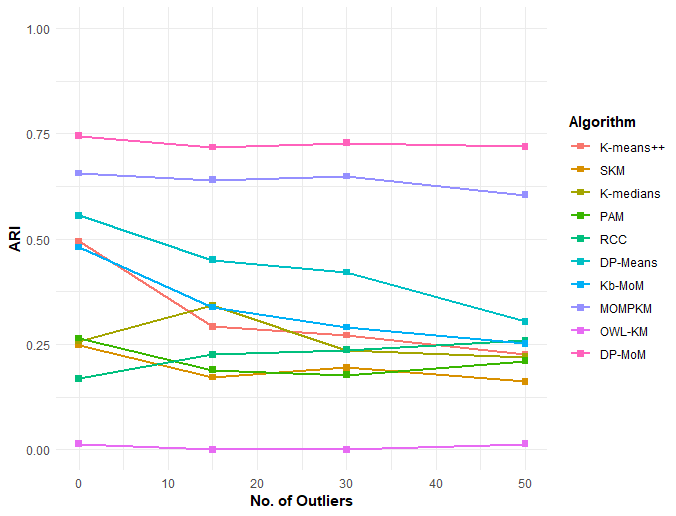
\includegraphics[width=0.4\textwidth]{Diagrams/plot-sim-ARI.png}
    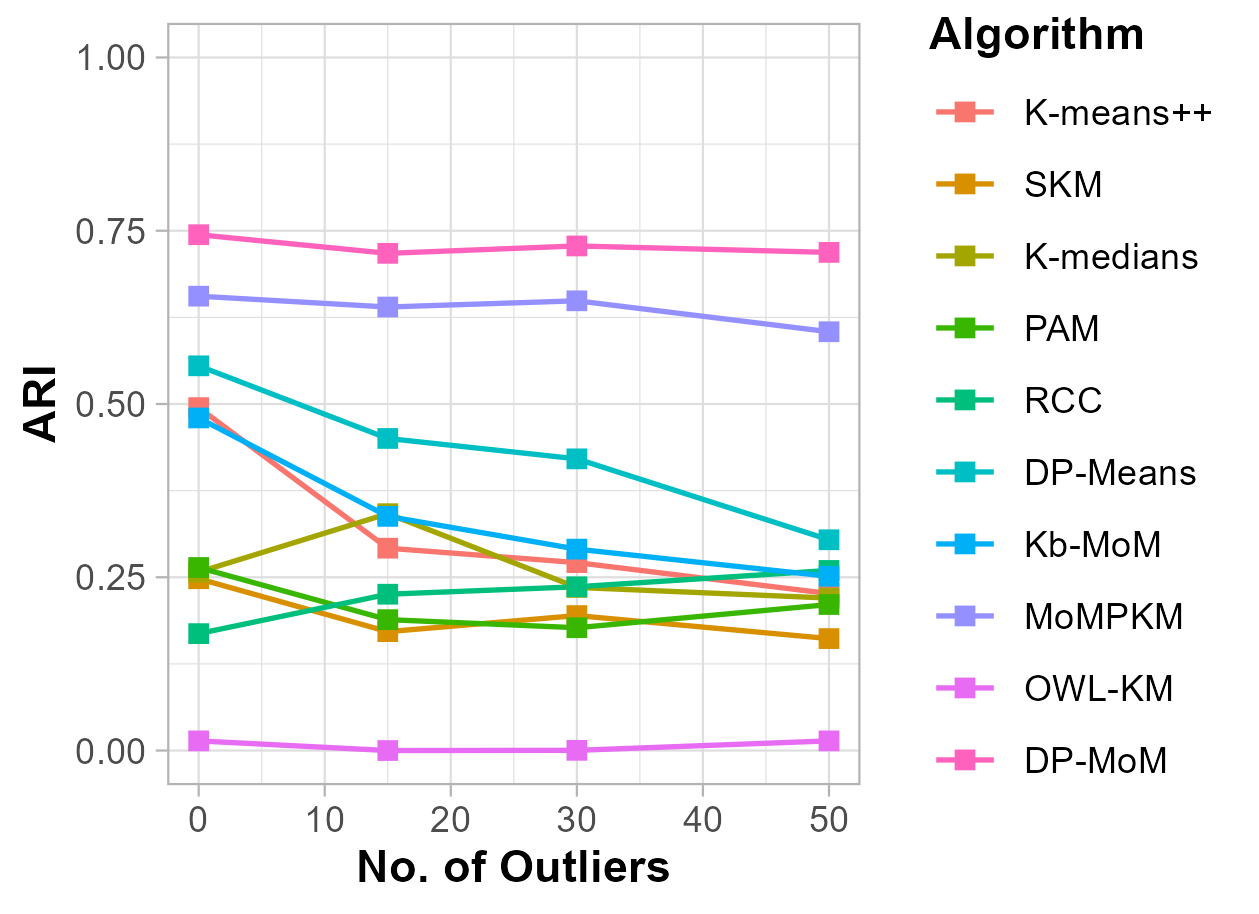
\includegraphics[width=0.5\textwidth]{Diagrams/plot-ari-sim-light-0.6.png}
    \caption{Line plots of ARI produced by different algorithms on simulated datasets, for increasingly higher number of outliers. DP-MoM is observed to perform uniformly better than all the competing methods.}
    \label{fig:plot-sim-ari}
\end{figure}

\begin{table*}[!htb]
\renewcommand\theadfont{\bfseries}
\centering
\caption{ARI values corresponding to clustering via state-of-the-art algorithms as well as DP-MoM on Compcancer datasets}
% \vskip 1em
\resizebox{\linewidth}{!}{
\begin{tabular}{lccccccccccccc}
\toprule
\multirow[b]{2}{*}{\thead{\textbf{Dataset}}}
    &   \multicolumn{3}{c}{\thead{\textbf{Description}}}
        & \multicolumn{9}{c}{\thead{\textbf{State-of-the-Art Algorithms}}}
             & \multirow[b]{2}{*}{\thead{\textbf{DP-MoM}}}\\
\cmidrule(lr){2-4}\cmidrule(lr){5-13} %\cmidrule(lr){11-13}
% \toprule
% & $\mathbf{n}$ & $\mathbf{d}$ & $\mathbf{K}$ & \thead{KM++} & \thead{DPM} & \thead{KMed} & \thead{PAM} & \thead{K-bMoM} & \\
& \textit{\textbf{n}} & \textit{\textbf{p}} & \textit{\textbf{K}} & \thead{KM++} & \thead{SKM} & \thead{KMed} & \thead{PAM} & \thead{RCC} & \thead{DPM} & \thead{KbMoM} & \thead{MoMPKM} & \thead{OWL-KM}  & %\thead{DP-MoM}
\\
% \addlinespace
\midrule
\addlinespace
golub\_1999\_v2     & 72         & 1868                  & 3                  & 0.4334          & 0.6876    & 0.6116          & 0.7716    & 0.0000            & 0.6421         & 0.5664   & 0.6361       & 0.7438            & \textbf{0.7798} \\
west\_2001          & 49         & 1198                  & 2                  & 0.1527          & 0.0002    & 0.0886          & 0.1058    & 0.0000            & 0.1715         & 0.3061   & 0.4761       & \textbf{0.5613}   & 0.5035           \\
pomeroy\_2002\_v2   & 42         & 857                   & 5                  & 0.0000                  & 0.4924    & 0.0000                  & 0.0000            & 0.0000            & 0.0514         & 0.3583   & 0.4685       & 0.5175            & \textbf{0.5446} \\
singh\_2002         & 102        & 339                   & 2                  & 0.0259           & 0.0330   & 0.0259           & 0.0330    & 0.0000            & 0.0574         & 0.0330  & 0.3433       & 0.0483           & \textbf{0.8135} \\
tomlins\_v2         & 92         & 1288                  & 4                  & 0.1418          & 0.1245    & 0.0100          & 0.2134    & 0.0000            & 0.1814           & 0.1730   & 0.2775       & 0.1993            & \textbf{0.3985} \\
alizadeh\_2000\_v1  & 42         & 1095                  & 2                  & 0.0127          & 0 .0000           & 0.0000                  & 0.2564    & 0.0000            & 0.0023         & 0.0613   & 0.2714      & 0.0889             & \textbf{0.3716}  \\
armstrong\_2002\_v2 & 72         & 2194                  & 3                  & 0.5123          & 0.5448     & 0.6625          & 0.4584    & 0.0000            & 0.4660         & 0.4992   & 0.6365       & \textbf{0.9186} & 0.8332          \\
bredel\_2005        & 50         & 832                   & 3                  & 0.2000          & 0.3525    & 0.0098          & 0.4760    & 0.0000            & 0.0893         & 0.2315   & 0.4877       & 0.2996            & \textbf{0.5841}\\
\addlinespace
\midrule
Average Rank        &          &                    &                   & 7.2500          & 6.0000  & 7.7500 & 5.3125          & 9.6875    & 5.8750            & 5.7500         & 3.1250          &  3.0000           & \textbf{1.2500}\\
\bottomrule
\end{tabular}}
\label{table:compcancer}
\end{table*}


\begin{table*}[!htb]
\renewcommand\theadfont{\bfseries}
\centering
\caption{ARI values corresponding to clustering via state-of-the-art algorithms as well as DP-MoM on UCI datasets}
% \vskip 1em
\resizebox{\linewidth}{!}{
\begin{tabular}{lccccccccccccc}
\toprule
\multirow[b]{2}{*}{\thead{\textbf{Dataset}}}
    &   \multicolumn{3}{c}{\thead{\textbf{Description}}}
        & \multicolumn{9}{c}{\thead{\textbf{State-of-the-Art Algorithms}}}
             & \multirow[b]{2}{*}{\thead{\textbf{DP-MoM}}}\\
\cmidrule(lr){2-4}\cmidrule(lr){5-13} %\cmidrule(lr){11-13}
% \toprule
% & $\mathbf{n}$ & $\mathbf{d}$ & $\mathbf{K}$ & \thead{KM++} & \thead{DPM} & \thead{KMed} & \thead{PAM} & \thead{K-bMoM} & \\
& \textit{\textbf{n}} & \textit{\textbf{p}} & \textit{\textbf{K}} & \thead{KM++} & \thead{SKM} & \thead{KMed} & \thead{PAM} & \thead{RCC} & \thead{DPM} & \thead{KbMoM} & \thead{MoMPKM} & \thead{OWL-KM}  & %\thead{DP-MoM}
\\
% \addlinespace
\midrule
\addlinespace
Iris           & 150  & 4  & 3 & 0.7237 & 0.7960 & 0.7515 & 0.6325 & 0.8090 & 0.7515          & 0.7565 & 0.8647          & 0.6339  & \textbf{0.9799}  \\
Glass          & 214 & 9  & 7 & 0.3728 & 0.3595 & 0.3367 & 0.3501 & 0.3930 & \textbf{0.4472} & 0.3467 & 0.2484          & 0.2659 & 0.3190          \\
WDBC           & 569 & 30 & 2 & 0.4223 & 0.4223 & 0.4603 & 0.4587 & 0.4146 & 0.4479          & 0.4560 & \textbf{0.6839} & 0.5897 & 0.6798           \\
E.Coli         & 336 & 7  & 8 & 0.5001 & 0.4918 & 0.5346 & 0.5407 & 0.5350 & 0.6663          & 0.6216 & 0.4952          & 0.2174 & \textbf{0.7835} \\
Wine           & 178 & 13 & 3 & 0.4140 & 0.4287 & 0.4226 & 0.4189 & 0.3564 & 0.4094          & 0.4227 & 0.5518          & 0.3470 & \textbf{0.5820} \\
Thyroid        & 215 & 5  & 3 & 0.3936 & 0.2145 & 0.1450 & 0.2144 & 0.5186 & 0.4971          & 0.3032 & 0.5995          & 0.4392  & \textbf{0.8842} \\
Zoo            & 101 & 16 & 7 & 0.7376 & 0.7516 & 0.6730 & 0.6566 & 0.7173 & 0.8270          & 0.4978 & 0.7603          & 0.8408 & \textbf{0.8477} \\
soybean & 47 & 35 & 4 & 0.7143 & 0.7138 & 0.7108 & 0.7437 & 0.8268 & 0.7368          & 0.82678 & 0.7417          & 0.5452 & \textbf{0.9533} \\
\addlinespace
\midrule
Average Rank        &          &                    &                   & 6.5625          & 6.1875  & 6.9375 & 6.5000          & 5.1875    & 4.6875            & 5.4375         & 4.2500          &  7.2500           & \textbf{2.0000}\\
\bottomrule
\end{tabular}}
\label{table:uci}
\end{table*}

\subsection{Real Data Experiments}

\subsubsection{Introducing Outliers - A Case Study}

We have picked the dataset \textit{Jain} \citep{jain-dataset} for this experiment. \textit{Jain} is a $2$-dimensional dataset with $373$ data points. The $2$ natural clusters are shaped like boomerangs, as can be seen in Figure 1 in Section \ref{sec:intro}. The performance of the algorithms was assessed on the original dataset. Afterward, several outliers were uniformly generated throughout the range of the data. $20$ fresh outliers were introduced in each of $4$ stages and at each stage, the algorithms were pitted against each other again. Even with the introduction of $80$ outliers, DP-MoM remained remarkably robust, consistently achieving a clustering accuracy of nearly $0.9$ in terms of ARI  (while the maximum ARI achieved was above that figure in all but one stage). Conversely, many other competing algorithms struggled to maintain their performance in the face of increasing outlier counts. They exhibited significant fluctuations in ARI as the number of outliers rose. Even the ones that maintained stability could only muster a measly ARI of $0.42$, as did all the other competing techniques.

\begin{figure}[!htb]
    \centering
    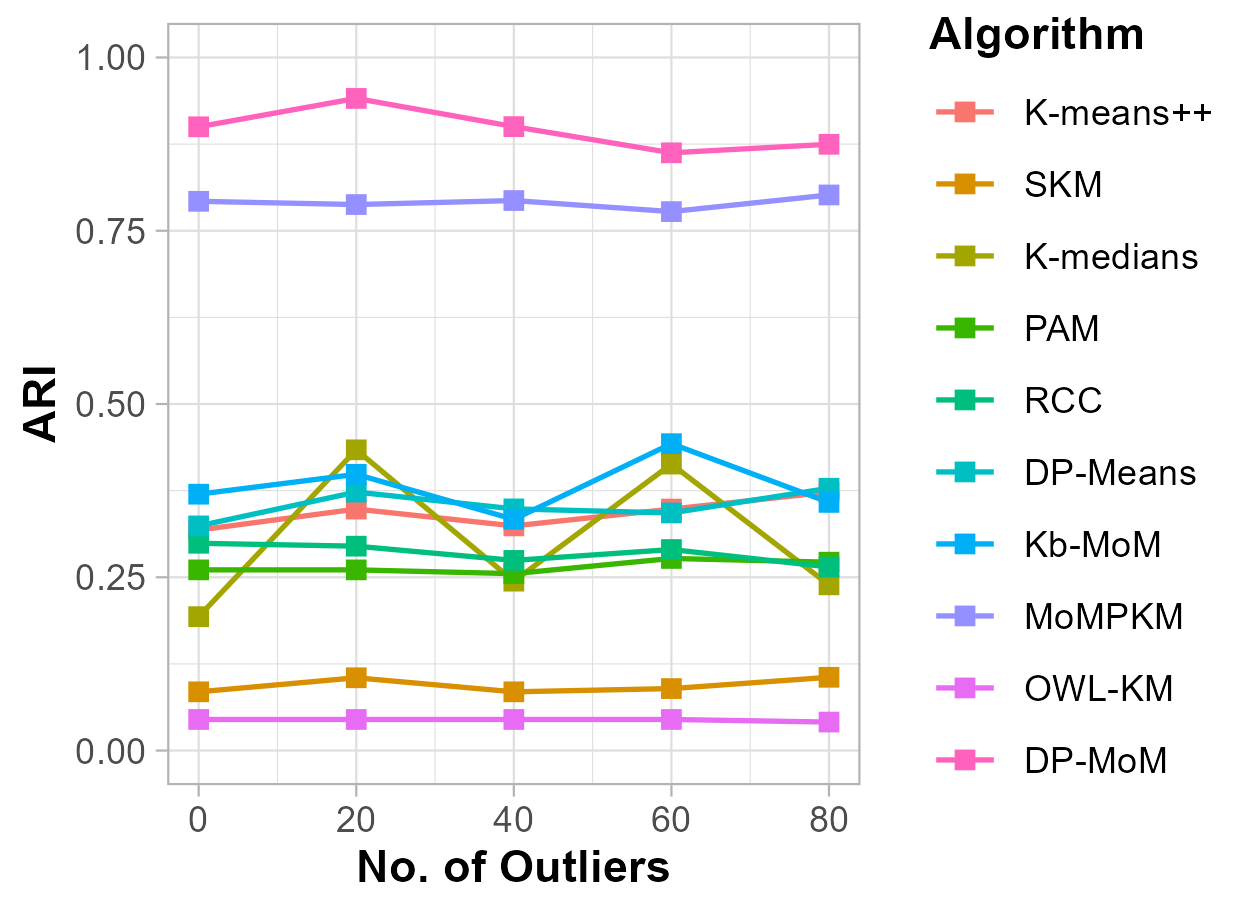
\includegraphics[width=0.45\textwidth]{Diagrams/plot-ari-jain-light-0.6.png}
    \caption{Line plots of ARI produced by different algorithms, for increasingly higher number of noisy observations introduced in the \textit{Jain} dataset. DP-MoM performs better than all the competing methods.}
    \label{fig:plot-jain-ari}
\end{figure}

\subsubsection{Further Experiments}

For a comprehensive performance evaluation of our proposed clustering algorithm in situations where the underlying data distributions are unknown, we implement DP-MoM on several real datasets from the Compcancer database and the UCI Repository. Additionally, we implement some state-of-the-art clustering algorithms mentioned at the start of this section, on the same datasets, and compare the corresponding ARI values against that of DP-MoM. Since DP-MoM is a randomized algorithm in the sense that its cluster assignment is dependent on the initial dataset partitioning into buckets, we implement DP-MoM on each dataset $30$ times independently, and report the median ARI. The same procedure is followed while reporting the ARI values for the competing algorithms.

\subsubsection{Friedman's Rank Test} 

Friedman's rank test \citep{friedman} is employed to discern whether a significant difference exists in the performance of the algorithms applied to our datasets. This assessment unfolds across three stages. In the initial stage, the test encompasses all clustering algorithms under consideration. Moving to the second stage, the analysis omits DP-MoM while incorporating the other algorithms. In the third stage, both MoMPKM and DP-MoM are excluded from the test. The calculated p-values for these three stages are as follows: $1.57 \times 10^{-7}$, $0.0021$, and $0.0599$ respectively. The null hypothesis, which posits no significant variance in clustering accuracy among the tested algorithms, is rejected in the first and second stages. However, it is accepted in the third stage. This outcome underscores that MoMPKM and DP-MoM emerge as the most proficient clustering algorithms at our disposal. Further assessments indicate that MoMPKM is outperformed comprehensively by the novel DP-MoM. 

\subsubsection{Sign Test and Wilcoxon Signed Rank (WSR) Test}

We also perform the \textit{Sign Test} and \textit{Wilcoxon Signed Rank Test} to compare our proposed algorithm individually with every other competing algorithm mentioned in Tables 1 and 2 and check whether DP-MoM performs significantly better than each of the aforementioned state-of-the-art algorithms. It is evident from the $p$-values that the null hypotheses: $H_{0s}:$ The said algorithm is better than our proposed algorithm DP-MoM (\textit{Sign Test}) and $H_{0w}:$ The said algorithm is equivalent to our proposed framework DP-MoM (\textit{Wilcoxon's signed Rank Test}) are rejected in favor of the alternative $H_1:$ DP-MoM performs significantly better than the other state-of-the-art clustering algorithm in question for a test with level of significance $0.01$. In a majority of the cases, our proposed DP-MoM algorithm is the standout performer. However, in the 3 cases where its performance is slightly suboptimal with respect to that of MoMPKM and OWL $k$-means, the results of the statistical tests presented in Table 3, indicate that this drop in performance is not statistically significant at the specified level.

\begin{table}[!htb]
\renewcommand\theadfont{\bfseries}
\centering
\caption{Summary of the Statistical Test Results for level of significance $0.01$}
\vskip 0.7em
\resizebox{0.6\linewidth}{!}{
\begin{tabular}{lccccccccccccc}
\toprule
\multirow[b]{2}{*}{\thead{\textbf{Clustering Algorithm}}}
    &   \multicolumn{2}{c}{\thead{\textbf{Sign Test}}}
        & \multicolumn{2}{c}{\thead{\textbf{WSR Test}}}
             \\
\cmidrule(lr){2-3}\cmidrule(lr){4-5} %\cmidrule(lr){11-13}
% \toprule
% & $\mathbf{n}$ & $\mathbf{d}$ & $\mathbf{K}$ & \thead{KM++} & \thead{DPM} & \thead{KMed} & \thead{PAM} & \thead{K-bMoM} & \\
& \thead{Statistic} & \thead{\textit{\textbf{p}}-value}  & \thead{Statistic} & \thead{\textit{\textbf{p}}-value} 
\\
% \addlinespace
\midrule
\addlinespace
$k$-means ++           & 15  & 0.0002594  & 135 & 0.0000305   \\
Sparse $k$-means          & 15  & 0.0002594  & 135 & 0.0000305          \\
$k$-medians           & 15  & 0.0002594  & 135 & 0.0000305         \\
Partition Around Medoids        & 15  & 0.0002594  & 134 & 0.0000458 \\
Robust Continuous Clustering           & 15  & 0.0002594  & 135 & 0.0000305 \\
DP means       & 15  & 0.0002594  & 133 & 0.0000763 \\
Kb MoM          & 15  & 0.0002594  & 135 & 0.0000305 \\
MoM Power $k$-means & 15  & 0.0002594  & 135 & 0.0000305 \\
OWL $k$-means & 14  & 0.0020900  & 125 & 0.0008392\\
\addlinespace
\bottomrule
\end{tabular}
}
\label{table:statistical tests}
\end{table}

Tables 4 and 5 provide the range of the penalty parameter $\lambda$ that enables us to cluster each dataset more efficiently. The predicted number of clusters are also displayed. Note that the number of clusters have been calculated after assigning the data points in the clusters containing less than $3$ observations, to the nearest cluster containing at least $3$ observations. 


\begin{table}[!htb]
\renewcommand\theadfont{\bfseries}
\centering
\caption{Range of optimal $\lambda$ and estimated number of clusters for implementing DP-MoM on UCI datasets}
\vskip 1em
\resizebox{0.5\linewidth}{!}{
\begin{tabular}{lcc}
\toprule
{\thead{\textbf{Dataset}}}
    &   \multicolumn{1}{c}{\thead{\textbf{Range of Optimal $\lambda$}}}
        & \multicolumn{1}{c}{{\textbf{Estimated Clusters}}}\\
% \addlinespace
\midrule
\addlinespace
Iris          & 5.129 - 6.535  & 3 \\
Glass         & 4.207 - 18.841  &  6 \\
WDBC           & 2.5$\times 10^6$ - 6$\times 10^6$  & 2 \\
E. Coli       & 0.3008 - 0.3571  & 8 \\
Wine         &  3.78$\times 10^5$ - 3.93$\times 10^5$ & 2 \\
Thyroid       & 1769 - 2123  & 5 \\
Zoo          & 7.048 - 10.360  & 6 \\
soybean & 18.59 - 25.70  & 4 \\
\addlinespace
\bottomrule
\end{tabular}
}
\label{table:lambda-uci}
\end{table}


\begin{table}[!htb]
\renewcommand\theadfont{\bfseries}
\centering
\caption{Range of optimal $\lambda$ and estimated number of clusters for implementing DP-MoM on Compcancer datasets}
\vskip 1em
\resizebox{0.6\linewidth}{!}{
\begin{tabular}{lcc}
\toprule
{\thead{\textbf{Dataset}}}
    &   \multicolumn{1}{c}{\thead{\textbf{Range of Optimal $\lambda$}}}
        & \multicolumn{1}{c}{\thead{\textbf{Estimated Clusters}}}\\
% \addlinespace
\midrule
\addlinespace
golub\_1999\_v2          & 2.48$\times 10^9$ - 3.05$\times 10^9$ & 3   \\
west\_2001         & 1.77$\times 10^9$  - 3.11$\times 10^9$ &  2         \\
pomeroy\_2002\_v2           & 2.94$\times 10^9$ - 4.70$\times 10^9$ & 4         \\
singh\_2002       & 0.14$\times 10^9$ - 0.17$\times 10^9$ & 2 \\
tomlins\_v2         &  175.6 - 308.0 & 2 \\
alizadeh\_2000\_v1       & 762.8 - 780.0  & 2 \\
armstrong\_2002\_v2          & 5.85$\times 10^9$ - 7.08$\times 10^9$ & 3 \\
bredel\_2005 & 672.4 - 978.8  & 2 \\
\addlinespace
\bottomrule
\end{tabular}
}
\label{table:lambda-compcancer}
\end{table}


\section{Discussion}

In this article, we proposed a new clustering algorithm that tactfully integrates two major clustering paradigms, viz., centroid-based clustering and model-based clustering that is intended to perform  well on noisy or outlier-infested data. We utilize the Median-of-Means (MoM) estimator to deal with noise or outliers present in data, and a Bayesian non-parametric modelling ensures that the number of clusters need not be specified earlier. Unlike conventional clustering algorithms, which typically tackle only one of these challenges, our proposed algorithm adeptly tackles both at the same time. Following our comprehensive theoretical analysis of error rate bounds, augmented by extensive simulation studies and real-world data analysis, we showcase the superiority of our methods against some of the most prominent clustering techniques.
%\bibliographystyle{abbrvnat}
%\bibliographystyle{plainnat}
\bibliographystyle{apalike}
\bibliography{references}


%%%%%%%%%%%%%%%%%%%%%%%%%%%%%%%%%%%%%%%%%%%%%%%%%%%%%%%%%%%%
\appendix


\section{An Additional Lemma}

\begin{lemma}\label{lemma-bound-Psi}
    For all $\bm{x}\in [-M,M]^p$ and $\bm{\Theta}\in \mathscr{G}$, \[0\le \Psi(d_{\phi}(\bm{x},\bm{\theta}_1), d_{\phi}(\bm{x},\bm{\theta}_2),\cdots, d_{\phi}(\bm{x},\bm{\theta}_K) )\le 4M^2p.\]
    Consequently, $\sup_{f\in \mathcal{F}}\|f\|_{\infty}\le 4M^2p$.
\end{lemma}

\begin{proof}
%     From the non-negativity of $\Psi(.)$, we get that $\Psi(d_{\phi}(\bm{x},\bm{\theta}_1), d_{\phi}(\bm{x},\bm{\theta}_2),\cdots, d_{\phi}(\bm{x},\bm{\theta}_K) )\ge 0$ for every $x\in [-M,M]^p$ and $\bm{\Theta}\in [-M,M]^{k\times p}$. Now,\begin{align*}
%         &\Psi(d_{\phi}(\bm{x},\bm{\theta}_1), d_{\phi}(\bm{x},\bm{\theta}_2),\cdots, d_{\phi}(\bm{x},\bm{\theta}_K) )\\
%         &=\min_{1\le j\le K}\|\bm{x}-\bm{\theta}_j\|_2^2\\
%         & \le \max_{1\le j\le K}\|\bm{x}-\bm{\theta}_j\|_2^2\\
%         & \le 4M^2p
%     \end{align*}
    Firstly,
    \begin{equation*}
        \Psi(d_{\phi}(\bm{x},\bm{\theta}_1), d_{\phi}(\bm{x},\bm{\theta}_2),\cdots, d_{\phi}(\bm{x},\bm{\theta}_K) ) = \min_{1\le j\le K}\|\bm{x}-\bm{\theta}_j\|_2^2 \le \max_{1\le j\le K}\|\bm{x}-\bm{\theta}_j\|_2^2 \le 4M^2p.
    \end{equation*}

    Since $\bm{x}$ is arbitrary, the second part of the lemma follows immediately.
\end{proof}

\section{Proofs from Section \ref{sec:theory}}


\subsection{Proof of Theorem \ref{thm-2-diff-Pn-P}}

\begin{proof}
    From Lemma \ref{lemma-bound-Psi}, we see that $\sup_{f\in \mathcal{F}}\|f\|_{\infty}\le 4M^2p$. Thanks to Theorem 4.10 of \cite{wainwright_2019}, for any $\delta \in (0,1)$, with probability at least $1-\delta$, 
    \begin{align*}
        \sup_{f\in \mathcal{F}}|P_n f-Pf| &\le 2\cdot\mathcal{R}_n(\mathcal{F})+\sup_{f\in \mathcal{F}}\|f\|_{\infty}\sqrt{\frac{2\log(2/\delta)}{n}}\\
        &\le 96\sqrt{\pi}M^2(Kp)^{3/2}n^{-1/2}+4\sqrt{2}M^2p\log^{\tfrac{1}{2}}\left(\frac{2}{\delta}\right) n^{-1/2}.
    \end{align*}
\end{proof}


\subsection{Proof of Theorem \ref{thm-4-MoM}}

\begin{proof} 
We represent the empirical distribution of $\{\bX_i\}_{i \in B_\ell}$ by $P_{B_{\ell}}$. Fix $\epsilon>0$. We will first establish a concentration inequality on $\sup_{\bTheta \in \mathscr{G}} |\text{MoM}_L^n (f_{\bTheta}) - P f_{\bTheta} |$. To that end, we bound the probabilities of the events $\{\sup_{\bTheta \in \mathscr{G}}(\text{MoM}_L^n (f_{\bTheta}) - P f_{\bTheta}) >\epsilon\}$ and $\{\sup_{\bTheta \in \mathscr{G}}  ( P f_{\bTheta} - \text{MoM}_L^n (f_{\bTheta})) > \epsilon\}$ individually. Note that 
\begin{equation}
\sup_{\bTheta \in \mathscr{G}}\sum_{\ell = 1}^L \one\left\{(P-P_{B_\ell})f_{\bTheta} > \epsilon\right\} > \frac{L}{2} \implies \sup_{\bTheta \in \mathscr{G}} (P f_{\bTheta} - \text{MoM}_L^n (f_{\bTheta})) > \epsilon.
\end{equation}
To see this, suppose on the contrary that \[\sup_{\bTheta \in \mathscr{G}}  (P f_{\bTheta} - \text{MoM}_L^n (f_{\bTheta})) \le \epsilon\] but \[\sup_{\bTheta \in \mathscr{G}}\sum_{\ell = 1}^L \one\left\{(P-P_{B_\ell})f_{\bTheta} > \epsilon\right\} > \frac{L}{2}\]. 
Then for all $\bm{\Theta}\in \mathscr{G}$, we must have \[\sup_{\bTheta \in \mathscr{G}}\sum_{\ell = 1}^L \one\left\{(P-P_{B_\ell})f_{\bTheta} > \epsilon\right\} > \frac{L}{2}\] which implies that for all $\bm{\Theta}\in \mathscr{G}$ \[\sum_{\ell = 1}^L \one\left\{(P-P_{B_\ell})f_{\bTheta} \le \epsilon\right\} \ge \frac{L}{2} \implies \sum_{\ell = 1}^L \one\left\{(P-P_{B_\ell})f_{\bTheta} > \epsilon\right\} \le \frac{L}{2}\] which in turn implies that \[\sup_{\bTheta \in \mathscr{G}}\sum_{\ell = 1}^L \one\left\{(P-P_{B_\ell})f_{\bTheta} > \epsilon\right\} \le \frac{L}{2}\] which is a contradiction. Let $\varphi(t) = (t-1) \one\{1 \le t \le 2\} + \one\{t >2\}$ where $\one\{\cdot\}$ is the indicator function. Evidently,
\begin{equation}
    \label{eq6}
    \one\{t \ge 2\} \le \varphi(t) \le \one\{t \ge 1\}.
\end{equation} 
We observe that
\begingroup
\allowdisplaybreaks
\begin{align}
    \sup_{\bTheta \in \mathscr{G}}\sum_{\ell = 1}^L \one\left\{(P-P_{B_\ell})f_{\bTheta} > \epsilon\right\}
    % \le & \sup_{\bTheta \in \mathscr{G}}\sum_{\ell \in \cL} \one\left\{(P-P_{B_\ell})f_{\bTheta} > \epsilon\right\} + |\cO|\nonumber\\
    % \le & \sup_{\bTheta \in \mathscr{G}}\sum_{\ell \in \cL}  \varphi\left(\frac{2(P-P_{B_\ell})f_{\bTheta}}{\epsilon}\right) + |\cO|\nonumber\\
    & \le \sup_{\bTheta \in \mathscr{G}}\sum_{\ell \in \cL}  \E \varphi\left(\frac{2(P-P_{B_\ell})f_{\bTheta}}{\epsilon}\right)  + |\cO|\nonumber\\
    & ~+\sup_{\bTheta \in \mathscr{G}}\sum_{\ell \in \cL}  \bigg[ \varphi\left(\frac{2(P-P_{B_\ell})f_{\bTheta}}{\epsilon}\right)   - \E \varphi\left(\frac{2(P-P_{B_\ell})f_{\bTheta}}{\epsilon}\right)\bigg]. \label{eq01}
\end{align}
\endgroup
Towards bounding $\sup_{\bTheta \in \mathscr{G}}\sum_{\ell = 1}^L \one\left\{(P-P_{B_\ell})f_{\bTheta} > \epsilon\right\}$, we first bound $\E \varphi\left(\frac{2(P-P_{B_\ell})f_{\bTheta}}{\epsilon}\right)$. Note that
\begingroup
\allowdisplaybreaks
% \begin{align}
% \small 
%   \E \varphi\left(\frac{2(P-P_{B_\ell})f_{\bTheta}}{\epsilon}\right) 
%   \le  \E \left[ \one\left\{\frac{2(P-P_{B_\ell})f_{\bTheta}}{\epsilon} > 1 \right\}\right] \nonumber  = & \sP \left[ (P-P_{B_\ell})f_{\bTheta}>\frac{\epsilon}{2} \right] \nonumber \\ 
%   \le & \exp\left\{-\frac{b \epsilon^2}{32 M^4 K^2 p^2}\right\}
% \end{align} 
\begin{equation*}
    \E \varphi\left(\frac{2(P-P_{B_\ell})f_{\bTheta}}{\epsilon}\right) \le  %\E \left[ \one\left\{\frac{2(P-P_{B_\ell})f_{\bTheta}}{\epsilon} > 1 \right\}\right] = 
    \sP \left[ (P-P_{B_\ell})f_{\bTheta}>\frac{\epsilon}{2} \right] \le \exp\left\{-\frac{b \epsilon^2}{32 M^4 K^2 p^2}\right\}.
\end{equation*}

The last inequality follows by Hoeffding's inequality after observing that $\displaystyle \mathbb{E} P_{B_{\ell}}f_{\bm{\Theta}}=Pf_{\bm{\Theta}}$ and by Lemma \ref{lemma-bound-Psi}.
\endgroup
 We now turn to bounding the term \[ \sup_{\bTheta \in \mathscr{G}}\sum_{\ell \in \cL}  \bigg[ \varphi\left(\frac{2(P-P_{B_\ell})f_{\bTheta}}{\epsilon}\right)   - \E \varphi\left(\frac{2(P-P_{B_\ell})f_{\bTheta}}{\epsilon}\right)\bigg]. \] Appealing to Theorem 26.5 of \cite{shalev-shwartz_ben-david_2014}, for all $ \bTheta \in \mathscr{G}$, we have
\begin{align}
  &\frac{1}{L}\sum_{\ell \in \cL}   \varphi\left(\frac{2(P-P_{B_\ell})f_{\bTheta}}{\epsilon}\right)- \E \left[\frac{1}{L}\sum_{\ell \in \cL}  \varphi\left(\frac{2(P-P_{B_\ell})f_{\bTheta}}{\epsilon}\right) \right]\nonumber \\
  &\le 2\E\left[\sup_{\bTheta \in \mathscr{G}}\frac{1}{L}\sum_{\ell \in \cL}\sigma_\ell  \varphi\left(\frac{2(P-P_{B_\ell})f_{\bTheta}}{\epsilon}\right) \right] + \delta.  \label{eq5}
\end{align}
with probability at least $1-2e^{-L\delta^2/2}$,
where $\{\sigma_\ell\}_{\ell \in \mathcal{L}}$ are i.i.d. Rademacher random variables independent of the sample $\mathcal{X}$. Consider i.i.d. Rademacher random variables $\{\xi_i\}_{i=1}^n$ independent of  $\{\sigma_\ell\}_{\ell \in \mathcal{L}}$. As a consequence of equation \eqref{eq5}, we get,  
\begingroup
\allowdisplaybreaks
\begin{align}
     & \frac{1}{L}\sup_{\bTheta \in \mathscr{G}}\sum_{\ell \in \cL}  \bigg[ \varphi\left(\frac{2(P-P_{B_\ell})f_{\bTheta}}{\epsilon}\right)  - \E \varphi\left(\frac{2(P-P_{B_\ell})f_{\bTheta}}{\epsilon}\right)\bigg] \nonumber\\
     & \le \frac{4}{L \epsilon}\E\left[\sup_{\bTheta \in \mathscr{G}}\sum_{\ell \in \cL}\sigma_\ell  (P-P_{B_\ell})f_{\bTheta} \right]+ \delta. \label{eq7} 
     \end{align}
     Equation \eqref{eq7} follows from the fact that $\varphi(\cdot)$ is 1-Lipschitz and Lemma 26.9 of \cite{shalev-shwartz_ben-david_2014}. We now consider random variables $\mathcal{X}^\prime=\{\bX_1^\prime, \dots, \bX_n^\prime\}$, which are i.i.d. and follow the law $P$. Equation \eqref{eq7} further yields
     \begin{align}
     = & \frac{4}{L \epsilon}\E\left[\sup_{\bTheta \in \mathscr{G}}\sum_{\ell \in \cL}\sigma_\ell  \E_{\mathcal{X}^\prime}\left((P^\prime_{B_\ell}-P_{B_\ell})f_{\bTheta}\right) \right]+ \delta \nonumber \\
     \le & \frac{4}{L \epsilon}\E\left[\sup_{\bTheta \in \mathscr{G}}\sum_{\ell \in \cL}\sigma_\ell  (P^\prime_{B_\ell}-P_{B_\ell})f_{\bTheta} \right]+ \delta \nonumber \\
     & \text{This inequality follows by employing Jensen's inequality as supremum is a convex function,}\nonumber\\ & \text{and the expectation in the second step is taken with respect to both the original sample $\mathcal{X}$}\nonumber\\ & \text{as well as the ghost sample $\mathcal{X}'$ and the Rademacher random variables $\{\sigma_{\ell}\}_{\ell\ge 1}$.}\nonumber\\
     = & \frac{4}{L \epsilon}\E\left[\sup_{\bTheta \in \mathscr{G}}\sum_{\ell \in \cL}\sigma_\ell  \frac{1}{b}\sum_{i \in B_\ell}(f_{\bTheta}(\bX_i^\prime)-f_{\bTheta}(\bX_i)) \right]+ \delta \nonumber \\
     = & \frac{4}{b L \epsilon}\E\left[\sup_{\bTheta \in \mathscr{G}}\sum_{\ell \in \cL}\sigma_\ell  \sum_{i \in B_\ell} \xi_i(f_{\bTheta}(\bX_i^\prime)-f_{\bTheta}(\bX_i)) \right]+ \delta \label{eq8} \\
     = & \frac{4}{n \epsilon}\E\left[\sup_{\bTheta \in \mathscr{G}}\sum_{\ell \in \cL}  \sum_{i \in B_\ell} \sigma_\ell \xi_i(f_{\bTheta}(\bX_i^\prime)-f_{\bTheta}(\bX_i)) \right]+ \delta \nonumber \\
     = & \frac{4}{n \epsilon}\E\left[\sup_{\bTheta \in \mathscr{G}} \sum_{i \in \J} \gamma_i (f_{\bTheta}(\bX_i^\prime)-f_{\bTheta}(\bX_i)) \right]+ \delta \label{eq9} \\
     \le &  \frac{4}{n \epsilon}\E\left[\sup_{\bTheta \in \mathscr{G}} \sum_{i \in \J} \gamma_i f_{\bTheta}(\bX_i^\prime)+ \sup_{\bTheta \in \mathscr{G}} \sum_{i \in \J} \gamma_i f_{\bTheta}(\bX_i) \right]+ \delta\\
     \le & \frac{4}{n \epsilon}\E\left[\sup_{\bTheta \in \mathscr{G}} \sum_{i \in \J} \gamma_i f_{\bTheta}(\bX_i^\prime)\right]+\E\left[ \sup_{\bTheta \in \mathscr{G}} \sum_{i \in \J} \gamma_i f_{\bTheta}(\bX_i) \right]+ \delta\\
     = & \frac{8}{n \epsilon}\E\left[\sup_{\bTheta \in \mathscr{G}} \sum_{i \in \J} \gamma_i f_{\bTheta}(\bX_i) \right]+ \delta \nonumber \\
     \le & \frac{8}{n \epsilon} 48 \sqrt{\pi}  M^2  (Kp)^{3/2}  \sqrt{|\J|} + \delta \label{eq10} \\
     \le & \frac{384}{n \epsilon}  \sqrt{\pi}  M^2  (Kp)^{3/2} \sqrt{|\I|} + \delta. \label{eq11}
\end{align}
\endgroup

Here $\J$ is the set of observations in the partitions not containing an outlier. Equation \eqref{eq8} follows from the fact that  $(f_{\bTheta}(\bX_i^\prime)-f_{\bTheta}(\bX_i)) \overset{d}{=} \xi_i(f_{\bTheta}(\bX_i^\prime)-f_{\bTheta}(\bX_i))$ as $\{\xi_i\}_{i\ge 1}$ are Rademacher random variables independent of the sample $\mathcal{X}$. In equation \eqref{eq9}, $\{\gamma_i\}_{i \in \mathcal{J}}$ are independent Rademacher random variables since the product of two independent Rademacher random varibles is also a Rademacher random variable. Equation \eqref{eq10} follows by Theorem \ref{thm-1-RnF}.
Thus, combining equations \eqref{eq5}, \eqref{eq7}, and \eqref{eq11}, we conclude that,  with probability of at least $1-2e^{-L \delta^2/2}$, 
\begin{equation}
    \sup_{\bTheta \in \mathscr{G}}\sum_{\ell = 1}^L \one\left\{(P-P_{B_\ell})f_{\bTheta} > \epsilon\right\} \le  L \left( \exp\left\{-\frac{b \epsilon^2}{32  M^4 K^2 p^2}\right\}+ \frac{|\cO|}{L} + \frac{384}{n \epsilon}  \sqrt{\pi} M^2  (Kp)^{3/2} \sqrt{|\I|} + \delta\right). \label{eq12}
\end{equation}
We choose $\delta = \frac{2}{4+\eta} - \frac{|\cO|}{L}$, and $$\epsilon = \max\left\{\sqrt{32  M^4 \log\left(\frac{4(\eta+4)}{\eta}\right)}KpL^{1/2}n^{-1/2}, \frac{1536(\eta+4)  M^2 \sqrt{\pi}}{\eta} (Kp)^{3/2} |\I|^{1/2}n^{-1}\right\}.$$ This makes the right hand side of \eqref{eq12} strictly smaller than $\frac{L}{2}$.
% In the unusual situation where you want a paper to appear in the
% references without citing it in the main text, use \nocite
%\nocite{langley00}
Thus, we have shown that 
\begin{align*}
     \sP\left( \sup_{\bTheta \in \mathscr{G}} (Pf_{\bTheta} - \text{MoM}^n_L (f_{\bTheta}))> \epsilon \right) \le 2e^{-L \delta^2/2}.
 \end{align*}
% \begin{align*}
%     &P\left( \sup_{\bTheta \in \mathscr{G}} (Pf_{\bTheta} - \text{MoM}^n_L (f_{\bTheta}))> \epsilon \right) \\
%     & \le P\left(\sup_{\bTheta \in \mathscr{G}}\sum_{\ell = 1}^L \one\left\{(P-P_{B_\ell})f_{\bTheta} > \epsilon\right\} \ge L/2\right) \le e^{-2L \delta^2}.
% \end{align*}
By a similar argument, it follows that,
\begin{align*}
    \sP\left( \sup_{\bTheta \in \mathscr{G}} (\text{MoM}^n_L (f_{\bTheta}) -Pf_{\bTheta} ) > \epsilon \right) \le 2e^{-L \delta^2/2}.
\end{align*}
From the two aforementioned inequalities, we obtain, 
\[\sP\left( \sup_{\bTheta \in \mathscr{G}} |\text{MoM}^n_L (f_{\bTheta}) -Pf_{\bTheta} | > \epsilon \right) \le 4e^{-L \delta^2/2}.\]
i.e., with at least probability $1-4e^{-L \delta^2/2}$,
\begin{align*}
    & \sup_{\bTheta \in \mathscr{G}} |\text{MoM}^n_L (f_{\bTheta}) -Pf_{\bTheta} | \\
    &\le \max\left\{\sqrt{32  M^4 \log\left(\frac{4(\eta+4)}{\eta}\right)}KpL^{1/2}n^{-1/2}, \frac{1536(\eta+4)  M^2 \sqrt{\pi}}{\eta} (Kp)^{3/2} |\I|^{1/2}n^{-1}\right\}\\
    &\lesssim \max\left\{ KpL^{1/2}n^{-1/2}, (Kp)^{3/2}  |\I|^{1/2}n^{-1}\right\}.
\end{align*}
\end{proof}



\end{document}
